\documentclass[12pt, a4paper,titlepage]{article}
\usepackage{appendix, pdfpages, float}
\usepackage{fullpage,graphicx,psfrag,amsmath,amsfonts,verbatim}
%use this package to set linespacing as desired
\usepackage{setspace}  
\singlespacing
\usepackage{subcaption}
\usepackage[euler]{textgreek}
\usepackage{titlesec}
\usepackage{tabularx}
%\usepackage[dvipsnames]{xcolor}
\usepackage{indentfirst}
\usepackage{multirow}

\titleformat
{\subsection}
{\normalfont\large\itshape}
{\thesubsection.}{0.5ex}{}

\titleformat
{\paragraph}[runin]
{\normalfont}
{}{0.5ex}{}

\graphicspath{{./images/}}

% Bibliography
%reference manager
\usepackage[backend=bibtex, sorting=none, style=numeric-comp, bibstyle=ieee]{biblatex}
\bibliography{biblio}
	
%%%%%%%%%%%%%%%%%%%%%%%%%%%%%%%%%%%%%%%%%%%%%%%%%%%%%%%%%%%%%%%%%%%%%%%%%%%%%%%
\begin{titlepage}
	\title{Dynamic Traffic Lights Management System Based On Traffic Flow Simulation With Performance Comparison of Various Smart Traffic Lights Technologies \vspace{1cm}\\Final Report}
	\author{Marcos Tulio Fermin Lopez\\Department of Electrical Engineering\\The City College of New York \vspace{2cm}\\Presented to Prof. Mohamed Ali}
	\date{Fall 2021}	
\end{titlepage}

%%%%%%%%%%%%%%%%%%%%%%%%%%%%%%%%%%%%%%%%%%%%%%%%%%%%%%%%%%%%%%%%%%%%%%%%%%%%%%%
\begin{document}
\maketitle
\newpage

\tableofcontents
\newpage
%%%%%%%%%%%%%%%%%%%%%%%%%%%%%%%%%%%%%%%%%%%%%%%%%%%%%%%%%%%%%%%%%%%%%%%%%%%%%%%
\section{Introduction}
\label{sec_intro}

Transportation Engineering studies the deployment of new technologies for the safe design, construction, and maintenance of transportation infrastructure. Some of these technologies implement novel ways to manage traffic, congestion, and urban mobility, with the help of artificial intelligence, computer vision, intelligent antennas, high-speed cameras, cloud computing, and IoT devices for real-time supervision. For example, as new ideas develop, traffic lights controllers are transitioning from static to dynamic systems. In general, a Dynamic Traffic Lights Controller is a system that adapts its timing according to the variations of traffic flow conditions instead of relying on a preprogrammed routine. 

In recent years government agencies and corporations in the Transportation Engineering field have dedicated resources to research methods for improving aging traffic lights systems to reduce the time drivers spend at intersections and promote smoother traffic flow. However, testing dynamic traffic lights controller designs can be costly, primarily when using state-of-the-art equipment that may not be readily available \cite{Jin17}. For this reason, researchers often rely on simulations of physical systems to test their designs and discover new opportunities for improvement at a low cost.
 
The simulation models proposed by researchers in \cite{Joyo20,Yaqub20} are of particular interest. In these simulations, traffic lights controllers use a smart mobile carrier antenna to communicate with the drivers' cellphones to determine the number of vehicles and their speed at a given intersection, improving the capabilities of previously installed traffic lights by adapting their timing based on traffic conditions.  In addition, simulation models test different traffic light timing configurations and create animations that illustrate how the model behaves \cite{Kamran17}.

Traffic flow modeling is essential to design conditions that provide drivers and pedestrians with a fast and enjoyable commute by solving congestion problems and producing more efficient traffic lights systems \cite{Wee13}. Multiple papers in the literature provide traffic flow simulations using statistical methods or dedicated open-source urban mobility simulation frameworks such as Eclipse SUMO, MATSim, NETSim and PTV Vissim \cite{Gartner92, Salimifard13}. An Arena 10 software simulation is proposed in \cite{Salimifard13} by solving a general traffic flow problem, treating the model as a discrete queuing system. In \cite{Gartner92}, a statistical method for evaluating alternative control strategies using NETSim is proposed using a pseudo-random number of cars. In both studies, simulation relies on certain conditions that may not be met at all times. The proposed methods also face challenges in practical implementation.

Although most papers in the literature propose simulation models using open-source software with a steep learning curve, very few of them design their own simulation software from scratch. However, sometimes it is more convenient to develop software that allows for a quicker implementation without compromising model accuracy and performance. Creating of a Python algorithm for simulating a microscopic traffic flow model with dynamic traffic lights based on traffic conditions can achieve a reliable environment for basic congestion analysis using either a high-speed camera, a smart antenna or a PIR sensor. Thus providing the fundamental principles of this research project. 

\newpage
%%%%%%%%%%%%%%%%%%%%%%%%%%%%%%%%%%%%%%%%%%%%%%%%%%%%%%%%%%%%%%%%%%%%%%%%%%%%%%%
\subsection{Contributions and Outline}

This research project proposes the microscopic simulation of a traffic flow model with Dynamic Traffic Lights using Pygame. The traffic lights timing self-adapts based on the traffic density at an arbitrary intersection. This project also evaluates the performance of a smart antenna, high-speed cameras, and PIR sensors as distinct traffic management technologies in the simulated environment. \\

The contributions of this simulation are the following:

\begin{enumerate}
	\item Creation of a microscopic traffic flow simulation in Python 3 using Pygame.
	\item Creation of a GUI.
	\item Creating a simulated environment that randomly generates cars, bikes, trucks, and buses at an arbitrary intersection. Allowing fundamental traffic flow analysis using three traffic management technologies.
	\item Design an algorithm for a Dynamic Traffic Lights Controller based on the traffic variations in the simulated traffic model, integrating a Smart Antenna, High-Speed Cameras, and PIR sensors and their respective logic.
	\item Performance evaluation of a smart antenna, high-speed cameras, and PIR sensors as distinct traffic management technologies in the simulated environment.
	\item Creation of tables and graphs demonstrating the simulation results in terms of the total number of cars served, the average waiting time at a red light, and efficiency for each technology.
	\item Reduction of daily commute time based on lower time waiting at an intersection and efficient traffic lights timing given the instantaneous traffic at the arbitrary intersection.
\end{enumerate}

This final report consists of 7 sections. The introduction presented above is section \ref{sec_intro}. Section \ref{sec_Methodology} provides a detailed explanation of the methods used to accomplish each simulation. Section \ref{sec_results} presents the results obtained after running the three simulations. Section \ref{sec_Conclusion} presents the conclusions and analysis of the obtained data. Section \ref{sec_future} presents ideas about future work that can be done to improve the project. Section \ref{sec_references} lists the references of this project. Finally, section \ref{sec_codes} contains a QR code to access the Github and python codes for this project.

\newpage
%%%%%%%%%%%%%%%%%%%%%%%%%%%%%%%%%%%%%%%%%%%%%%%%%%%%%%%%%%%%%%%%%%%%%%%%%%%%%%%
\section{Methodology}
\label{sec_Methodology}

This section details the methods, programming logic, and assumptions used to create the simulation environment and implement each traffic management technology.

The simulations developed in this project were written in Python programming language with the help of pygame as the main library. Pygame provides a set of modules that allow the creation of 2D video games integrating audio and graphics.

%%%%%%%%%%%%%%%%%%%%%%%%%%%%%%%%%%%%%%%%%%%%%%%%%%%%%%%%%%%%%%%%%%%%%%%%%%%%%%%
\subsection{Graphical User Interface}
\label{subsec_gui}

To provide a simple method of interacting with the simulations, a graphical user interface (GUI) was created. This GUI allows the user to access each simulation individually and plot the final data from a secondary menu. The final version of the GUI is provided below:

\begin{figure}[H]
	\centering
	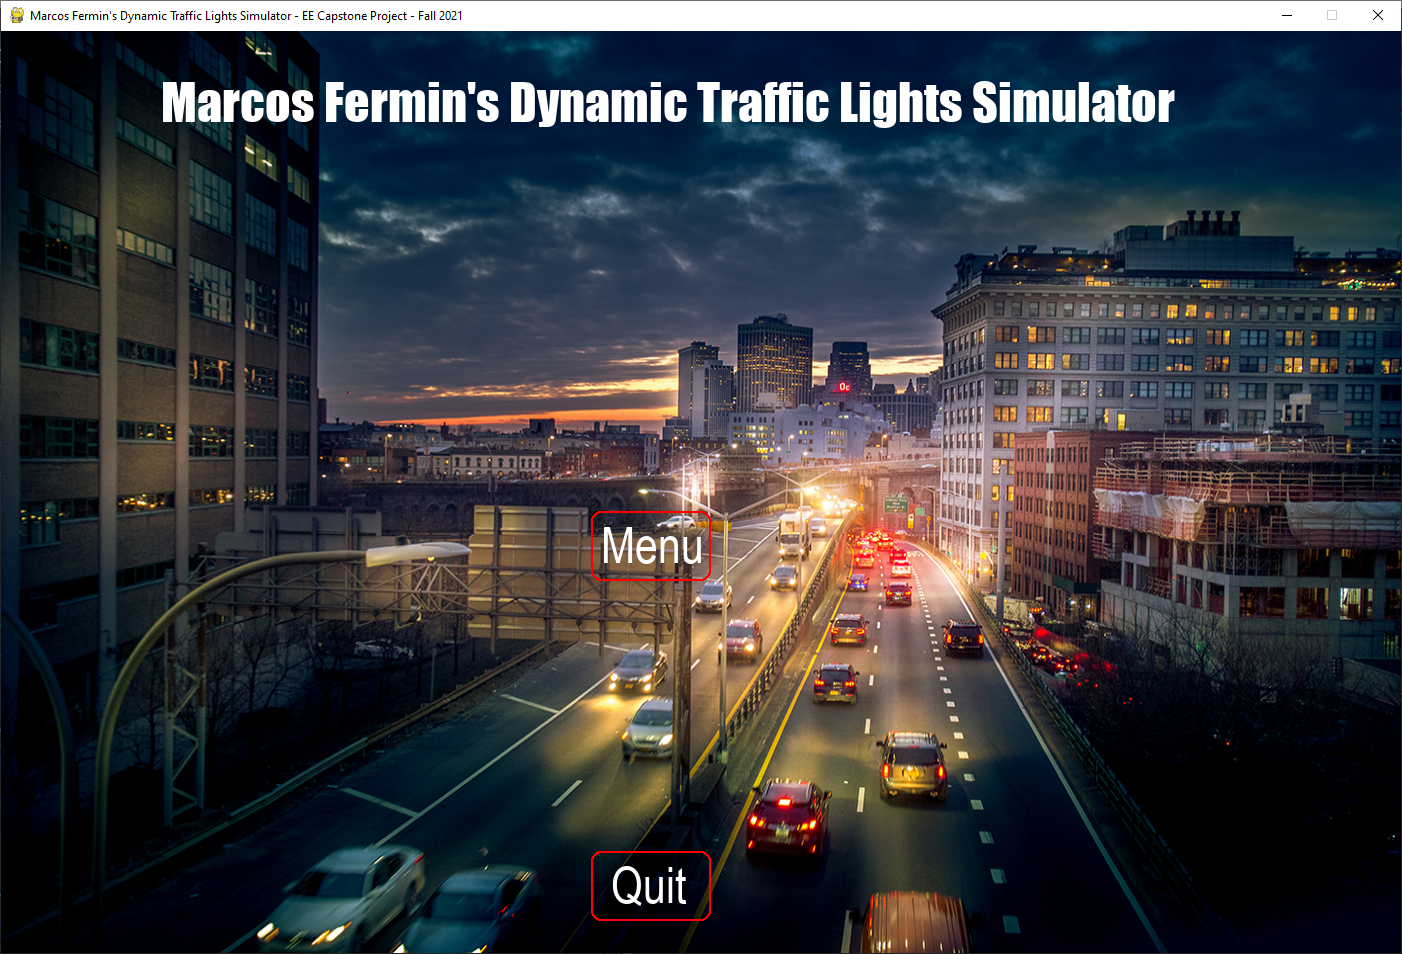
\includegraphics[width=\linewidth]{images/GUI_1}
	\caption{Main page of the graphical user interface.}
	\label{fig:gui1}
\end{figure}

After pressing the "Menu" button in figure \ref{fig:gui1}, the user is taken to a secondary page as shown in figure \ref{fig:gui2}, where each simulation can be launched in any order, and the available data can be plotted.

\begin{figure}[H]
	\centering
	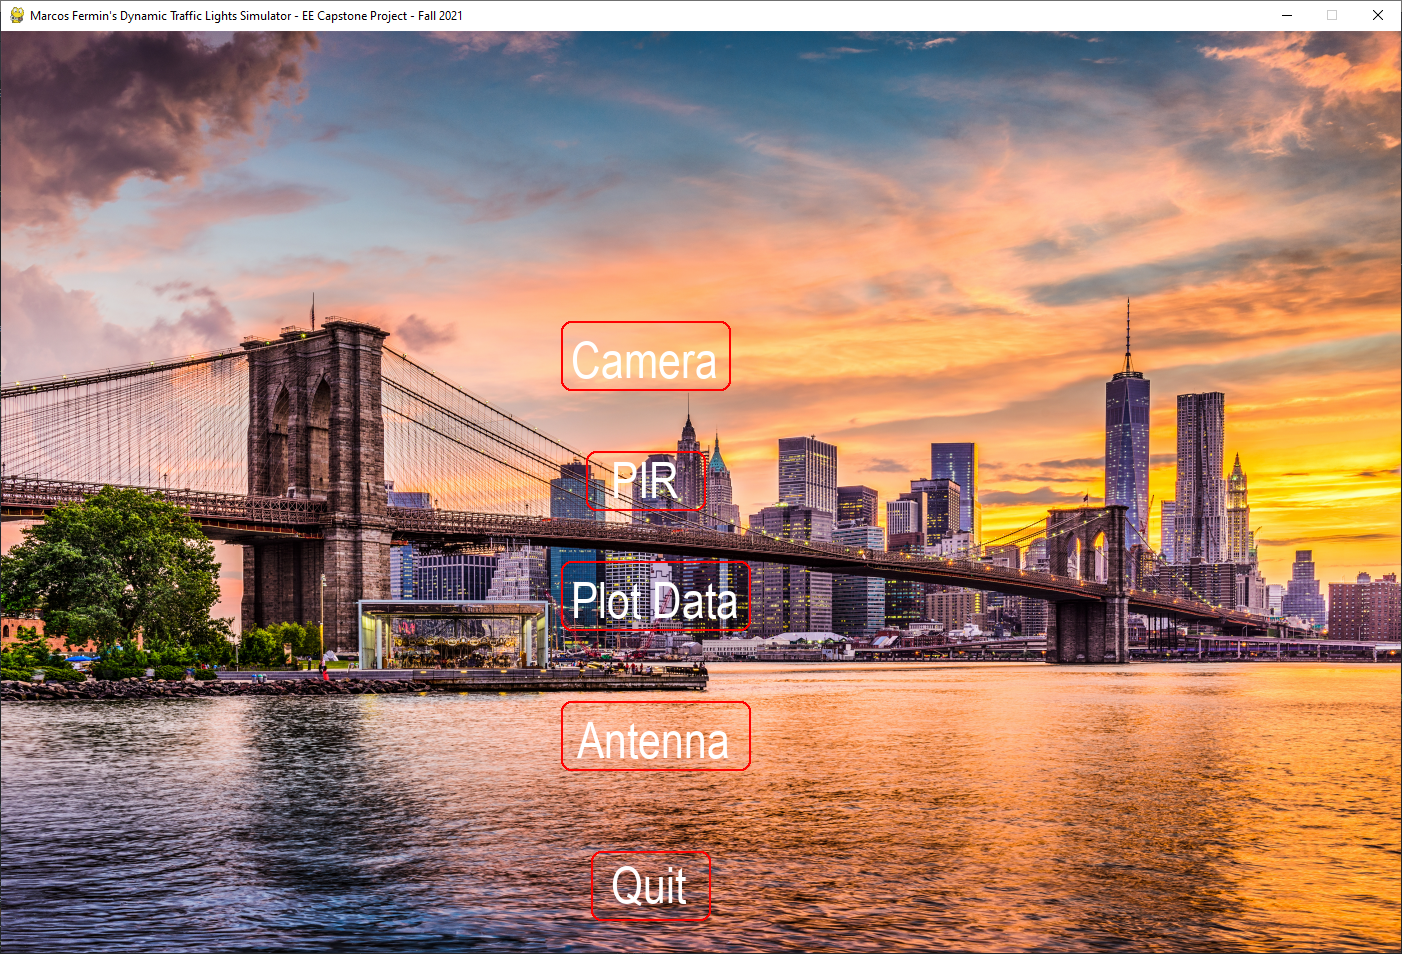
\includegraphics[width=\linewidth]{images/GUI_2}
	\caption{Secondary page of the graphical user interface.}
	\label{fig:gui2}
\end{figure}

\newpage
%%%%%%%%%%%%%%%%%%%%%%%%%%%%%%%%%%%%%%%%%%%%%%%%%%%%%%%%%%%%%%%%%%%%%%%%%%%%%%%
\subsection{Antenna Simulation}
\label{subsec_antenna}

This module simulates the Dynamic Traffic Lights with a smart antenna covering the intersection. The fundamental assumption for the smart antenna technology is to provide a highly efficient method to dynamically control traffic lights by exploiting the capabilities of the telecommunications antennas currently in use by mobile carriers. It determines the number of cars present in each direction of the intersection by summing the number of vehicles East to West and North to South that collide with each lane of the intersection.

The green light timing of each traffic light ranges from 60 to 180 seconds depending on the number of cars present. The antenna will verify the presence of vehicles in either direction every 60 seconds. If there are cars present in the opposite direction, the light will switch. In case there is no traffic in either direction the green lights will stay on for 180 seconds to then switch to the opposite direction, so on and so forth.

\begin{figure}[H]
	\centering
	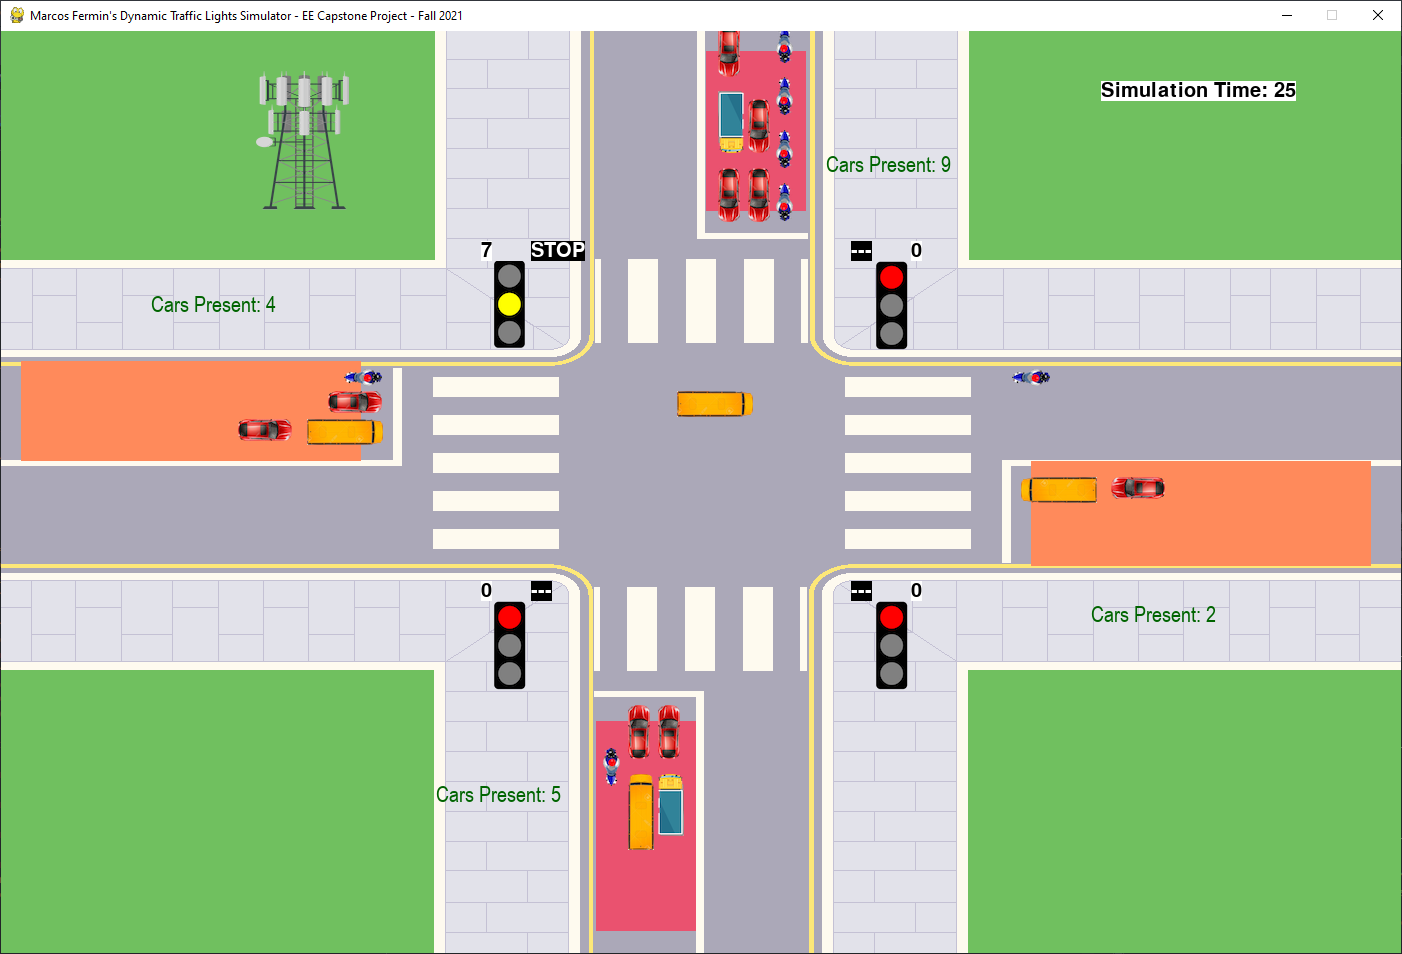
\includegraphics[width=\linewidth]{images/Antenna}
	\caption{Antenna Simulation Window}
	\label{fig:antenna}
\end{figure}

\subsubsection{Python Code Explanation}

\begin{figure}[H]
	\centering
	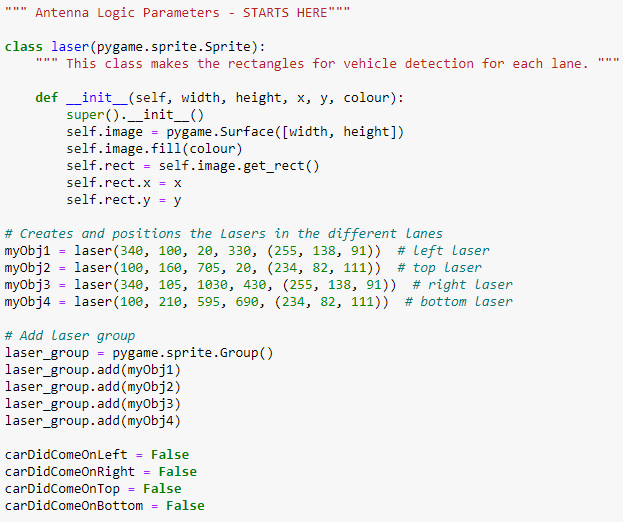
\includegraphics[width=\linewidth]{images/a1}
	\caption{}
	\label{fig:a1}
\end{figure}

As shown in figure \ref{fig:a1}, This class makes rectangles (referred to as Lasers, which represent the antenna's operating range in each direction) used for collision detection. We give the surface x,y coordinates to place it on the screen. 

Since we have four lanes, we make four laser-type objects and add them to the sprite group called "laser group." CarDidComeOnLeft, CarDidComeOnRight, CarDidComeOnTop and CarDidComeOnBottom are Booleans used to detect if a car did come onto a particular lane. They are initially false and set to true if vehicles collide with the corresponding laser or rectangle via the pygame.sprite.spritecollide function.

We then reset the booleans above in case a vehicle is not on the laser to clear the carDidCome variables. We check for collisions with the pygame.sprite.spritecollide function and if cars are present the variables are set true.

\begin{figure}[H]
	\centering
	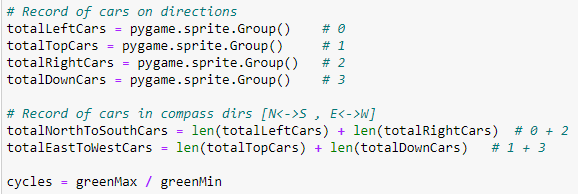
\includegraphics[width=\linewidth]{images/a2}
	\caption{}
	\label{fig:a2}
\end{figure}

We keep a count of total cars in each lane with the above variables. Total cars in each direction (North to South and East to West) are calculated by adding their respective lanes.

\begin{figure}[H]
	\centering
	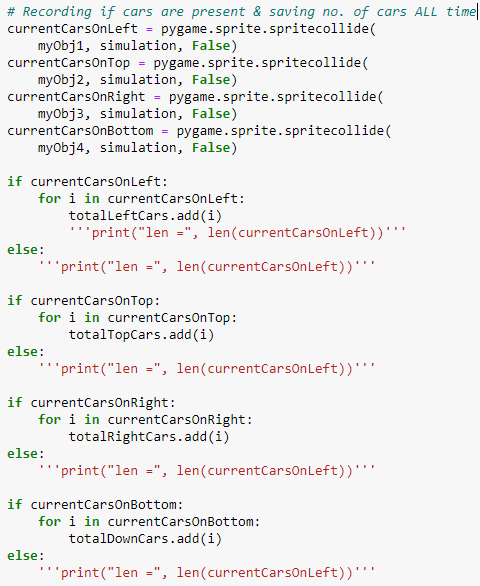
\includegraphics[width=\linewidth]{images/a3}
	\caption{}
	\label{fig:a3}
\end{figure}

When cars are on their respective lane which is detected by the lasers, we add that car into the total variable of that lane.

\begin{figure}[H]
	\centering
	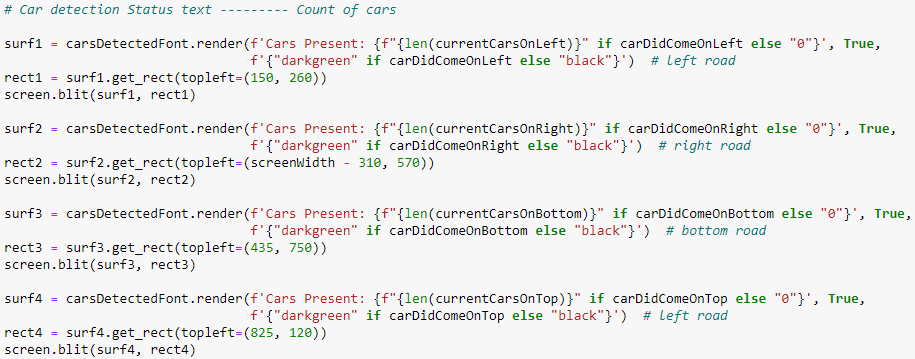
\includegraphics[width=\linewidth]{images/a4}
	\caption{}
	\label{fig:a4}
\end{figure}

We use the ternary operator along with carDidCome variables to change the detection font. We then go onto detection and switching logic for which we employ our f, cycle, carsDidCome and state variables to check the current state. State variable is used to check if we are either on the x-axis (0 – 2) lane or y-axis (1 - 3) lane.

\begin{figure}[H]
	\centering
	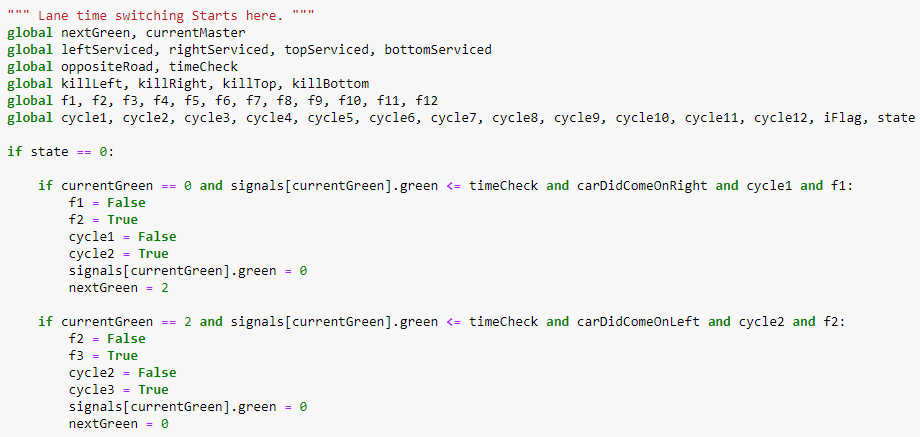
\includegraphics[width=\linewidth]{images/a5}
	\caption{}
	\label{fig:a5}
\end{figure}

\begin{figure}[H]
	\centering
	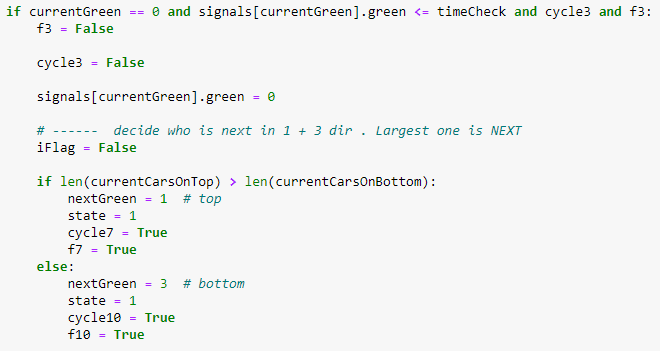
\includegraphics[width=\linewidth]{images/a6}
	\caption{}
	\label{fig:a6}
\end{figure}

\begin{figure}[H]
	\centering
	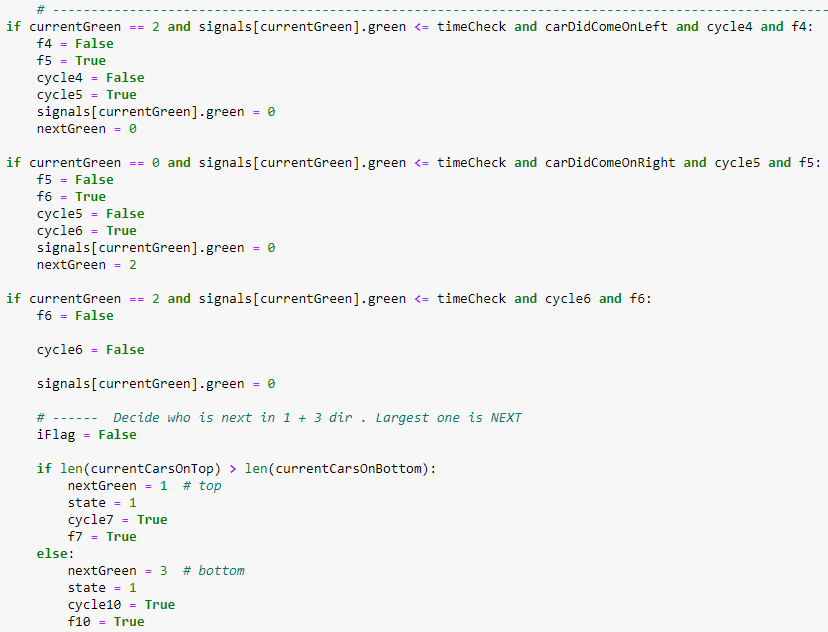
\includegraphics[width=\linewidth]{images/a9}
	\caption{}
	\label{fig:a9}
\end{figure}

As shown in figures \ref{fig:a5}, \ref{fig:a6} and \ref{fig:a9}, if the variable "state" is 0, we are at the x-axis serving lanes 0 and 2. Vehicles move in a lane until at least the greenMinTime has passed, and if cars are present in the opposite lane, we stop executing and go to the opposite lane and vice versa until greenMaxTime has passed.

We then continue to execute until an entire cycle has finished for the axis. A cycle is finished when there are three executions in that axis. We chose three executions since our greenMaxTime is 180 and greenMinTime is 60; hence: Cycles = 180/60 = 3

We check which lane will be executed next in the next axis when execution is finished. In this case, the axis will be y since our state was 0. Since we want the lane with more cars to execute, we check the length of the currentCars variable, then the one with the largest value will be our next lane to execute, adjusting the cycles and state flags appropriately.

Once we are executing the other axis and its three executions are over, we will check which lane in the other axis (x-axis) has more cars, and that will be our next lane to execute and so on.\\

\textbf{Traffic Lights' Switching Logic}:\\

We have two axes in our simulation, x, and y. The two comprise lanes 0, 2 for the x-axis and lanes 1,3 for the y-axis. We need to stay in one direction until greenMaxTime has run out. However, if other cars are in the opposing lane and greenMinTime has run out, we swap onto the other lane. Then we must wait until greenMinTime  has passed to check if cars are present in the lane, and if so, we switch back to the previous lane and execute it until greenMinTime and greenMaxTime run out.

We then have to go to the other axis and find out which lane has more cars. The lane with more cars will be our current lane, and we shall continue executing as before, waiting for Tmax to run out and if Tmin has passed and there are cars on the opposite lane, we will switch to that lane.

\newpage
%%%%%%%%%%%%%%%%%%%%%%%%%%%%%%%%%%%%%%%%%%%%%%%%%%%%%%%%%%%%%%%%%%%%%%%%%%%%%%%
\subsection{Camera Simulation}
\label{subsec_camera}

This module simulates the Dynamic Traffic Lights with a high speed camera in each direction. The fundamental assumption for the high speed camera technology is to provide a highly efficient image processing method to dynamically control traffic lights by detecting the presence of vehicles at the intersection. In a real-time IoT project the cameras would be connected to a image processing module that detects the vehicles using computer vision. However, for this simulation, only the expected behavior of the traffic lights after image processing was considered.

This module assumes that the cameras are sending their live feed to a image processing unit, and the traffic lights' timing self-adjust based on the processing done by this unit. The green light timing of each traffic light changes dynamically by providing a longer greentime to the direction that has the most vehicles. The signals are activated in a clock-wise direction.

\begin{figure}[H]
	\centering
	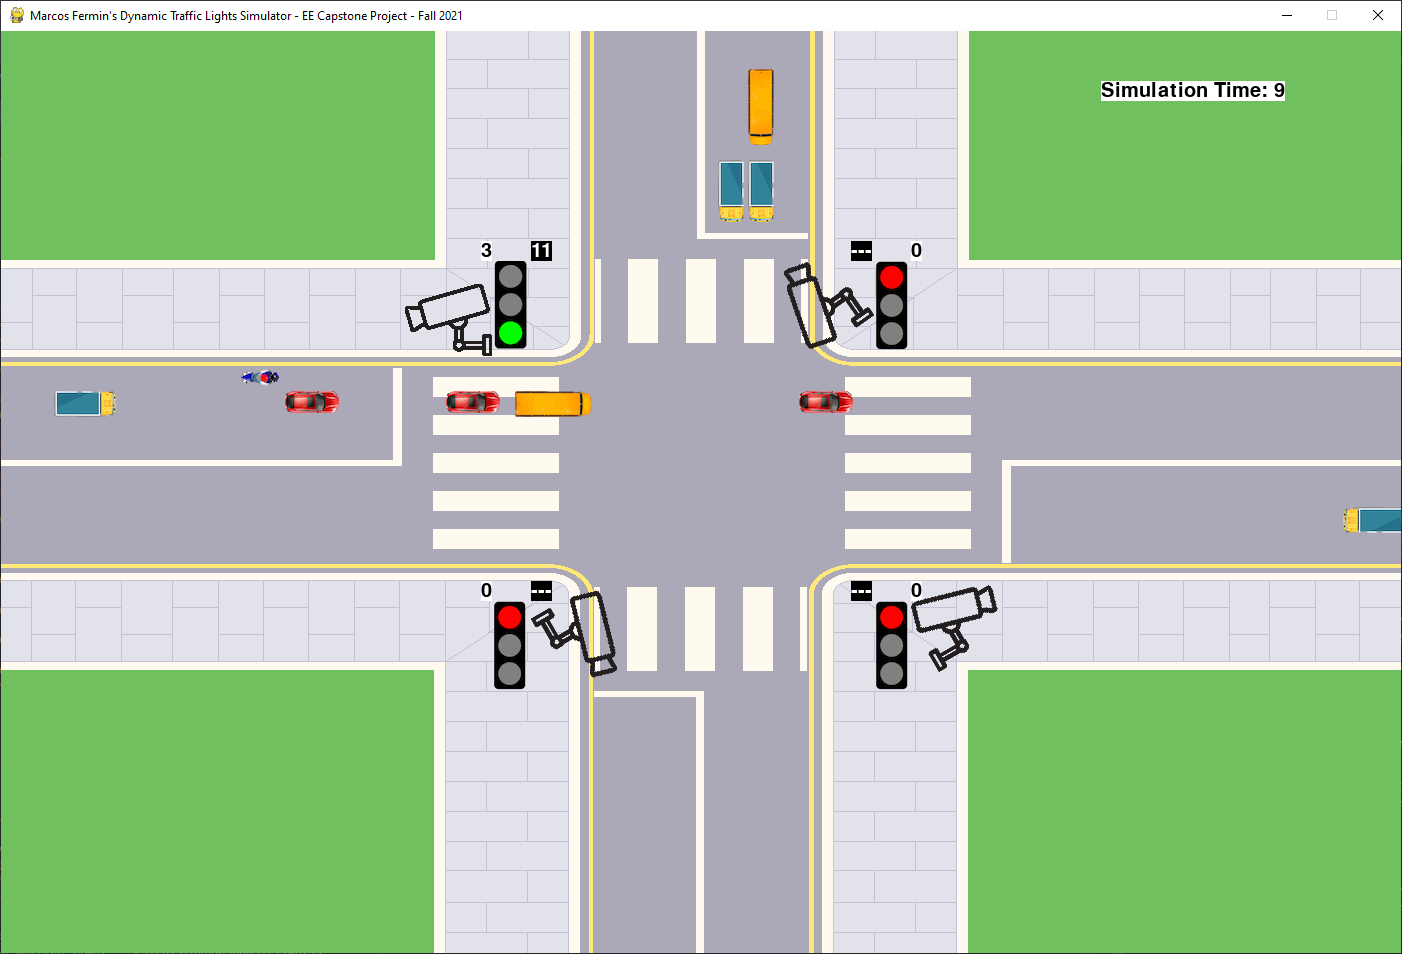
\includegraphics[width=\linewidth]{images/Camera}
	\caption{}
	\label{fig:camera}
\end{figure}

\subsubsection{Python Code Explanation}

\begin{figure}[H]
	\centering
	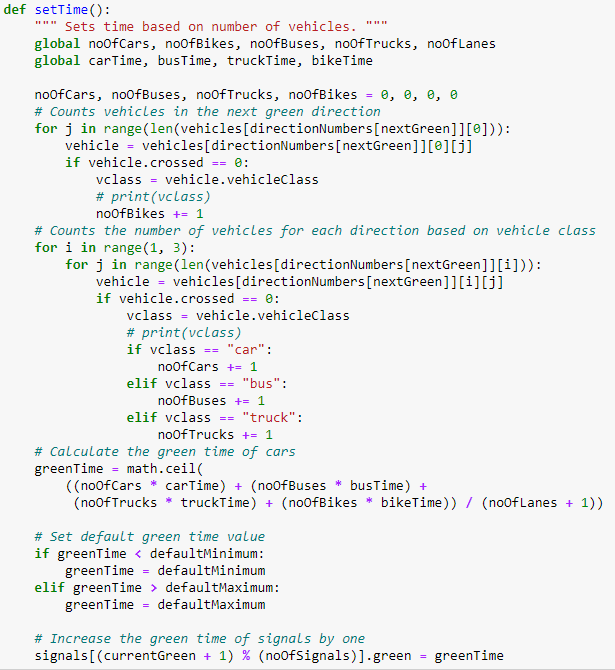
\includegraphics[width=\linewidth]{images/c3}
	\caption{}
	\label{fig:c3}
\end{figure}

As shown in figure \ref{fig:c3} above, the setTime() function defines the method used to determine the timing of the green lights based on the number of vehicles present at the intersection after being detected by the camera. First the algorithm counts the number of vehicles in the next green direction to allocate time according to the traffic density. Then it counts the number of vehicles for each direction based on vehicle class to determine how many vehicles of each class are detected by the camera at any given time. 

The green lights timing is calculated by using the following formula, using the ceiling function. The ceiling function f(x) takes a real number x as an input and returns the least integer greater than or equal to x:

\begin{figure}[H]
	\centering
	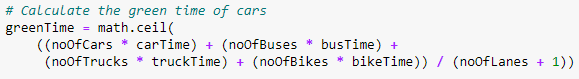
\includegraphics[width=\linewidth]{images/f1}
	\caption{Formula to calculate greenTime of camera}
	\label{fig:f1}
\end{figure}

\begin{figure}[H]
	\centering
	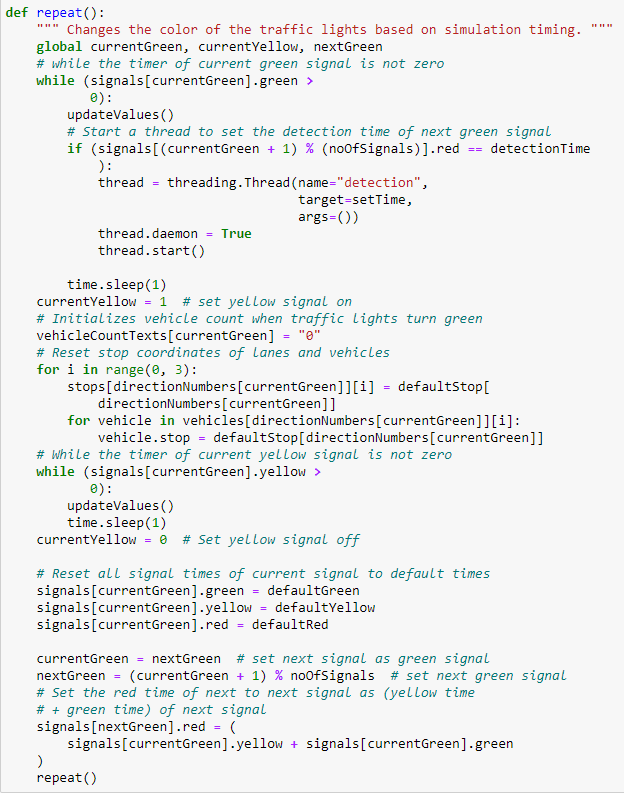
\includegraphics[width=\linewidth]{images/c4}
	\caption{}
	\label{fig:c4}
\end{figure}

\begin{figure}[H]
	\centering
	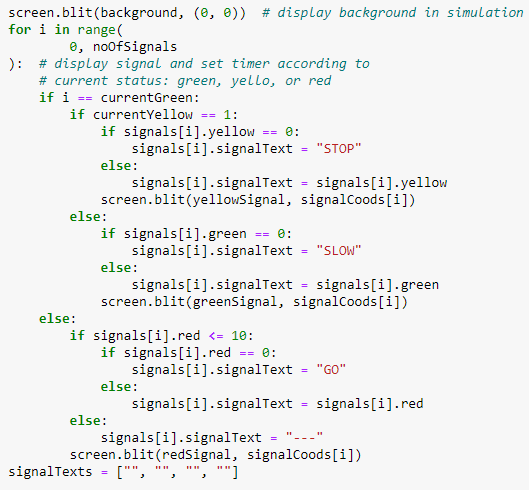
\includegraphics[width=\linewidth]{images/c1}
	\caption{}
	\label{fig:c1}
\end{figure}

As shown in figure \ref{fig:c1} above, we iterate over each of the signals and check if the one we are currently on is green. If it is, we check if its yellow time is 1 (which would mean it will switch to red in a second) and if so, we blit STOP as the signal text. If not, we blit the current yellow time.

If the current signal is not green, we check if its red timer is less than 10 seconds. If it is, we then check if the time is precisely 0, which would denote this is the signal that must be the next green signal and blit GO as the text. If the red timer's time is not less than or equal to 10, we blit the current red timer.

\begin{figure}[H]
	\centering
	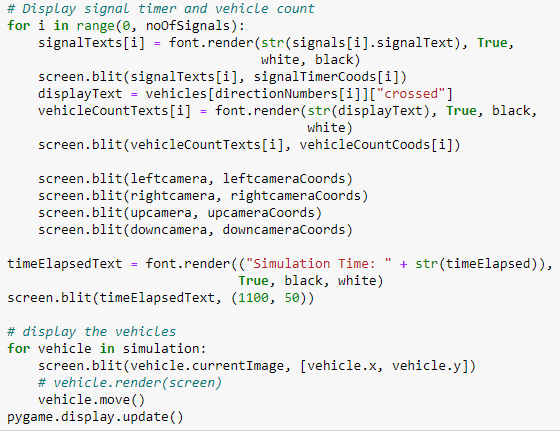
\includegraphics[width=\linewidth]{images/c2}
	\caption{}
	\label{fig:c2}
\end{figure}

We blit our texts and timers following the light switching logic, including our simulation time and vehicle crossed count. We then blit the camera images, moving each vehicle in our simulation sprite group called "move."\\

\textbf{Selection Logic}:\\

We start with signal [0] as our initial signal and the subsequent signals are calculated with the nextGreen variable which calculates by:
\begin{equation}\label{key}
	 (currentGreen+1) \, \% \, noOfSignals
\end{equation}

\newpage
%%%%%%%%%%%%%%%%%%%%%%%%%%%%%%%%%%%%%%%%%%%%%%%%%%%%%%%%%%%%%%%%%%%%%%%%%%%%%%%
\subsection{PIR Simulation}
\label{subsec_pir}

This module simulates the Dynamic Traffic Lights with PIR Sensors at the intersection. The fundamental assumption for the PIR Sensor technology is to provide a method of detecting the presence of cars based on movement in each direction of the intersection. In this simulation, the PIR sensors are represented by "rays" that detect the presence of vehicles when they "collide" with the rays within the sensors' operating range.

The PIR sensor logic is implemented following a "master-slave" module where East is lane 0, West is lane 2, North is lane 1 and South is lane 3. With this assumption the sensors check every greenmax if vehicles are present in the opposite direction.

\begin{figure}[H]
	\centering
	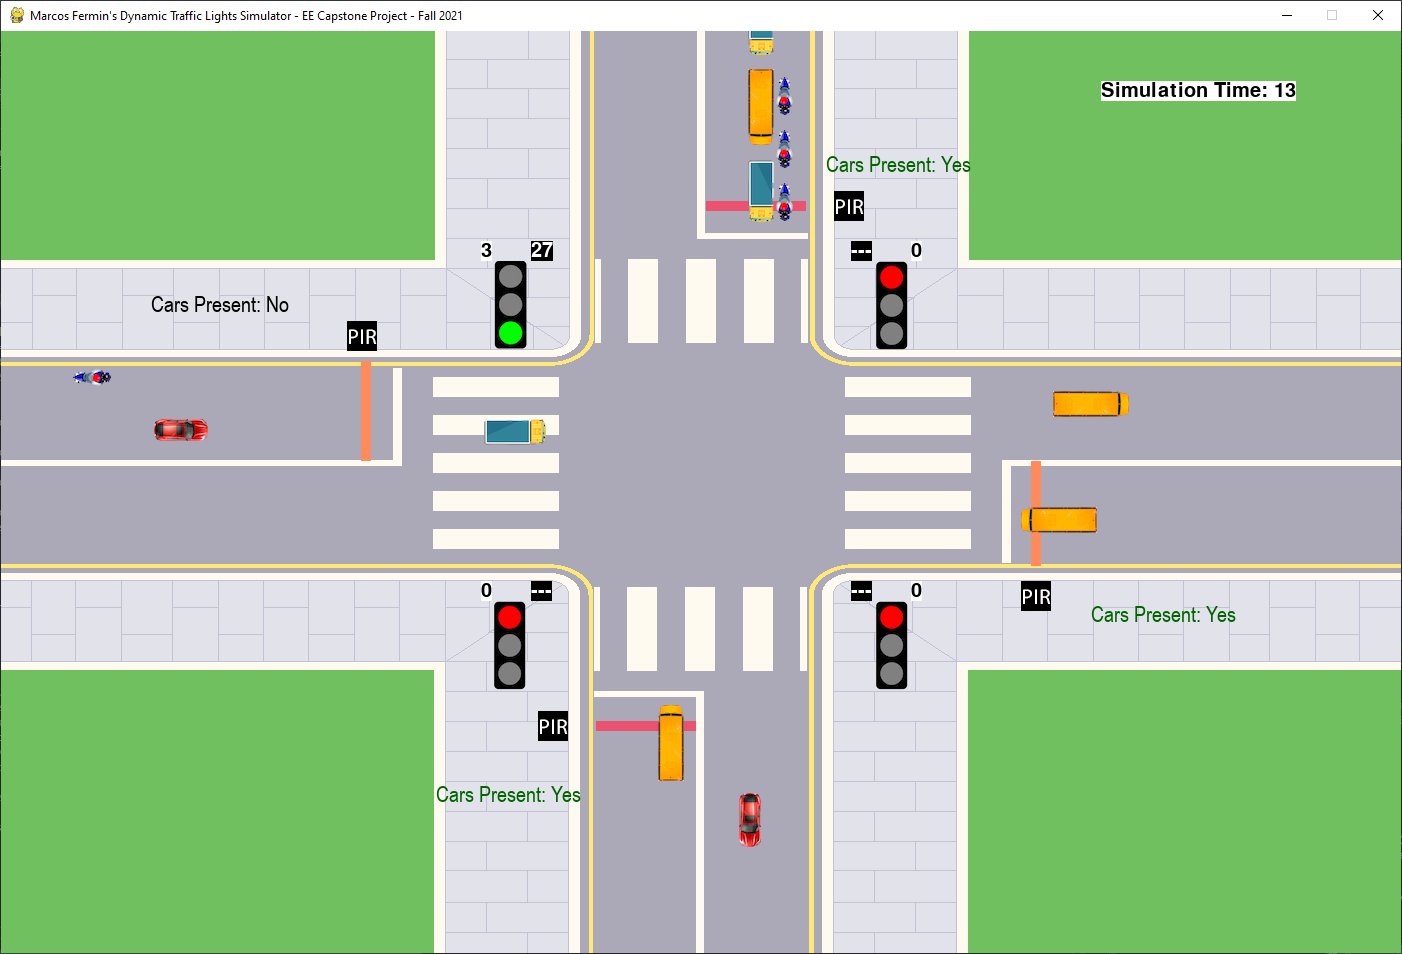
\includegraphics[width=\linewidth]{images/PIRsensor}
	\caption{}
	\label{fig:pirsensor}
\end{figure}

\subsubsection{Python Code Explanation}

\begin{figure}[H]
	\centering
	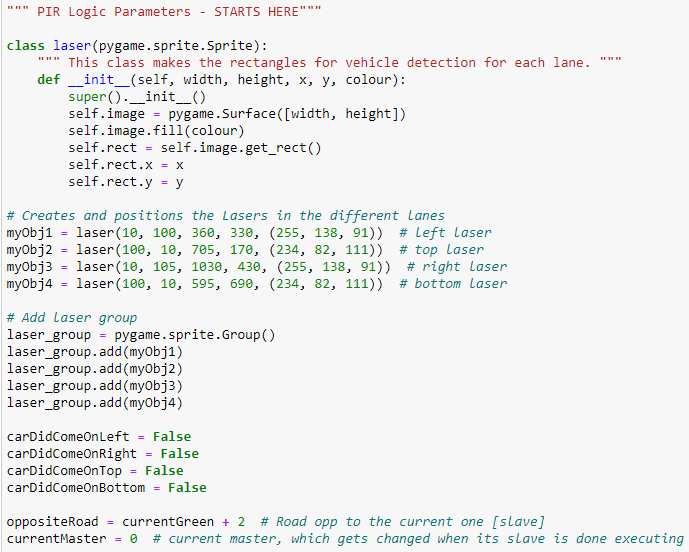
\includegraphics[width=\linewidth]{images/p1}
	\caption{}
	\label{fig:p1}
\end{figure}

As shown in figure \ref{fig:p1}, This class makes rectangles (referred to as Lasers, which represent the antenna's operating range in each direction) used for collision detection. We give the surface x,y coordinates to place it on the screen. 

Since we have four lanes, we make four laser-type objects and add them to the sprite group called "laser group." CarDidComeOnLeft, CarDidComeOnRight, CarDidComeOnTop and CarDidComeOnBottom are Booleans used to detect if a car did come onto a particular lane. They are initially false and set to true if vehicles collide with the corresponding laser or rectangle via the pygame.sprite.spritecollide function.

\begin{figure}[H]
	\centering
	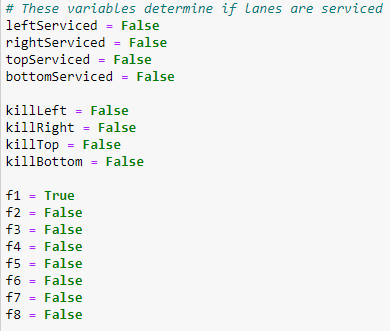
\includegraphics[width=\linewidth]{images/p2}
	\caption{}
	\label{fig:p2}
\end{figure}

Figure \ref{fig:p2} illustrates that leftServiced, rightServiced, topServiced, and bottomServiced are Booleans which determine if a lane has been serviced. A lane is serviced when the current lane and the lane opposite to it have finished execution. For example, if the current lane is left (0) and finishes execution for at least the greenMinTime the control gets transferred to the opposite lane right (2). When (2) has been serviced for at least the greenMinTime,  the left lane is said to be serviced. The f variables are used to lockout a lane for executing again. If the variable is false, that particular lane won’t be executable

\begin{figure}[H]
	\centering
	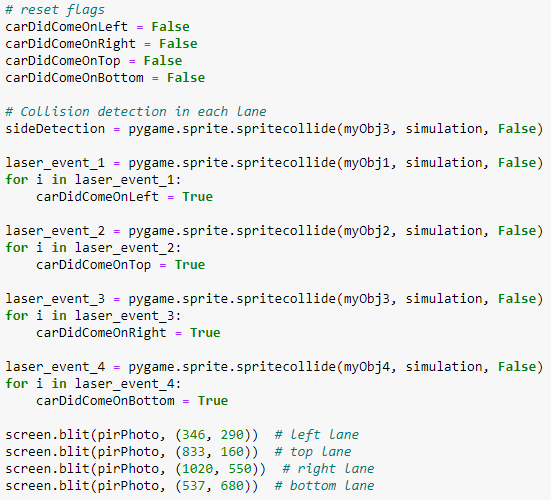
\includegraphics[width=\linewidth]{images/p3}
	\caption{}
	\label{fig:p3}
\end{figure}

We then reset the booleans above in case a vehicle is not on the laser to clear the carDidCome variables. We check for collisions with the pygame.sprite.spritecollide function and if cars are present the variables are set true.

\begin{figure}[H]
	\centering
	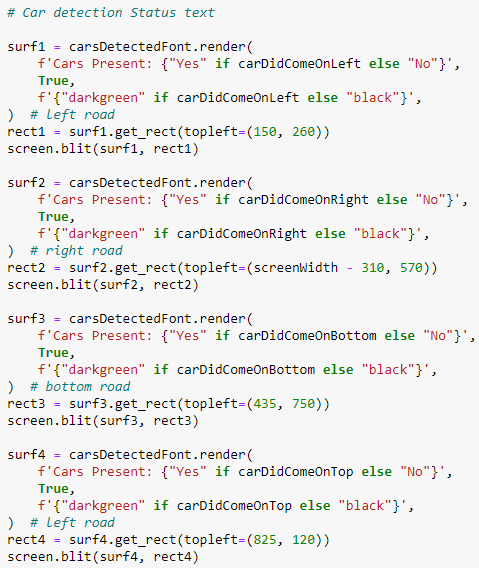
\includegraphics[width=\linewidth]{images/p4}
	\caption{}
	\label{fig:p4}
\end{figure}

Using the ternary operator and carDidCome variables if cars are present, we show Yes and if not, we show No as the text in Cars present. This process emulates the detection of movement sensed by the PIR sensors.

\begin{figure}[H]
	\centering
	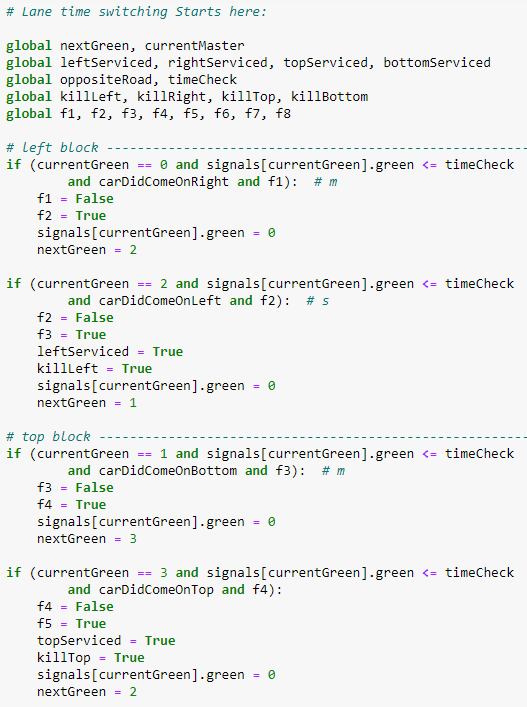
\includegraphics[width=\linewidth]{images/p5}
	\caption{}
	\label{fig:p5}
\end{figure}

\begin{figure}[H]
	\centering
	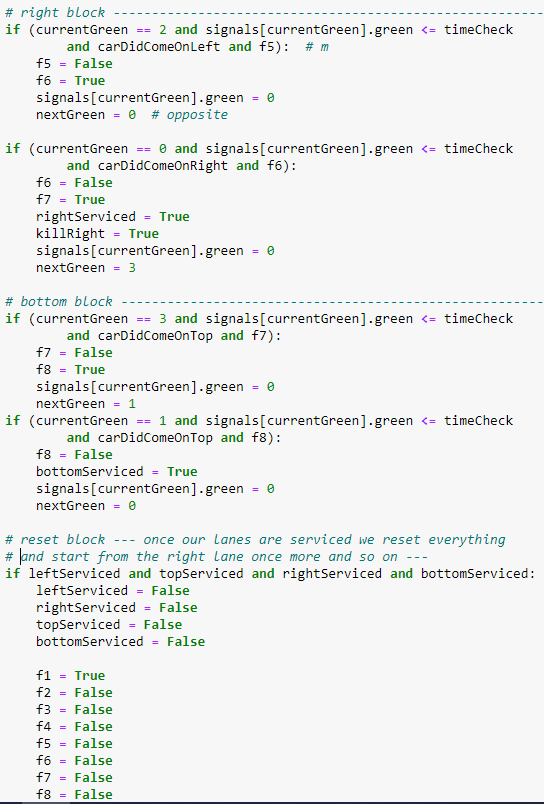
\includegraphics[width=\linewidth]{images/p6}
	\caption{}
	\label{fig:p6}
\end{figure}

As shown in figures \ref{fig:p5} and \ref{fig:p6}, we check every lane with its own block, which looks like the above. This block is used to check lane 0. Each lane gets greenMaxTime as its maximum green time. However, if there are vehicles in the opposing lane (initially lane 2), and greenMinTime has passed, we will stop executing the direction of current green. The opposing lane will then proceed to execute for greenMaxTime, or if vehicles are present in the opposite lane it will execute for greenMaxTime only. 

Once the opposite lane has been serviced, the lane is said to be serviced. In this case, the lane serviced will be lane 0. We will then check lane one and repeat the above process until we have serviced all lanes, at which point we will reset all flags so we can start executing from lane 0 again.\\

\textbf{PiR Switching Logic}:\\

Our main idea is to service a lane for at least greenMinTime if there are no cars in the opposite lane. To achieve this, we need to monitor the lane whose turn it is and the current executing lane. The current executing lane is the one that needs to be serviced. When the current lane and its opposing lane are executed, they are both considered "served." The current lane is the one that is currently executing (currently green).

We then choose a lane (0 in this case) as an example to explain the concept. First, we will let lane (0) execute for at least the greenMinTime; if greenMinTime finishes and there are no cars in the opposite lane until the time reaches 0, we will say lane 0 has been serviced and move onto the next lane in turn. However, if greenMinTime is finished and there are cars in the opposing lane, we will stop executing the current lane (0) and make the current lane equal to the opposite lane (lane two). 

When lane two's execution time reaches greenMinTime, we will detect if cars are in the opposite lane(lane 0). If there are cars in lane 0, we will stop executing lane two and say lane 0 is serviced, move onto the next lane in turn (1), and so on. If there are no cars in lane 0, we will keep executing lane two until the time runs out and move onto the next lane in turn.

\newpage
%%%%%%%%%%%%%%%%%%%%%%%%%%%%%%%%%%%%%%%%%%%%%%%%%%%%%%%%%%%%%%%%%%%%%%%%%%%%%%%
\section{Results and Data Analysis}
\label{sec_results}

This section presents the results obtained after running the three simulations for 1 hour (3600 seconds).

In this project, a traffic flow simulated environment that randomly generates cars, bikes, trucks, and buses at an arbitrary intersection was created. Allowing fundamental traffic flow analysis using three traffic management technologies. The performance of these three technologies was compared based on the total number of cars served and the average waiting time at red lights.

\begin{figure}[H]
	\centering
	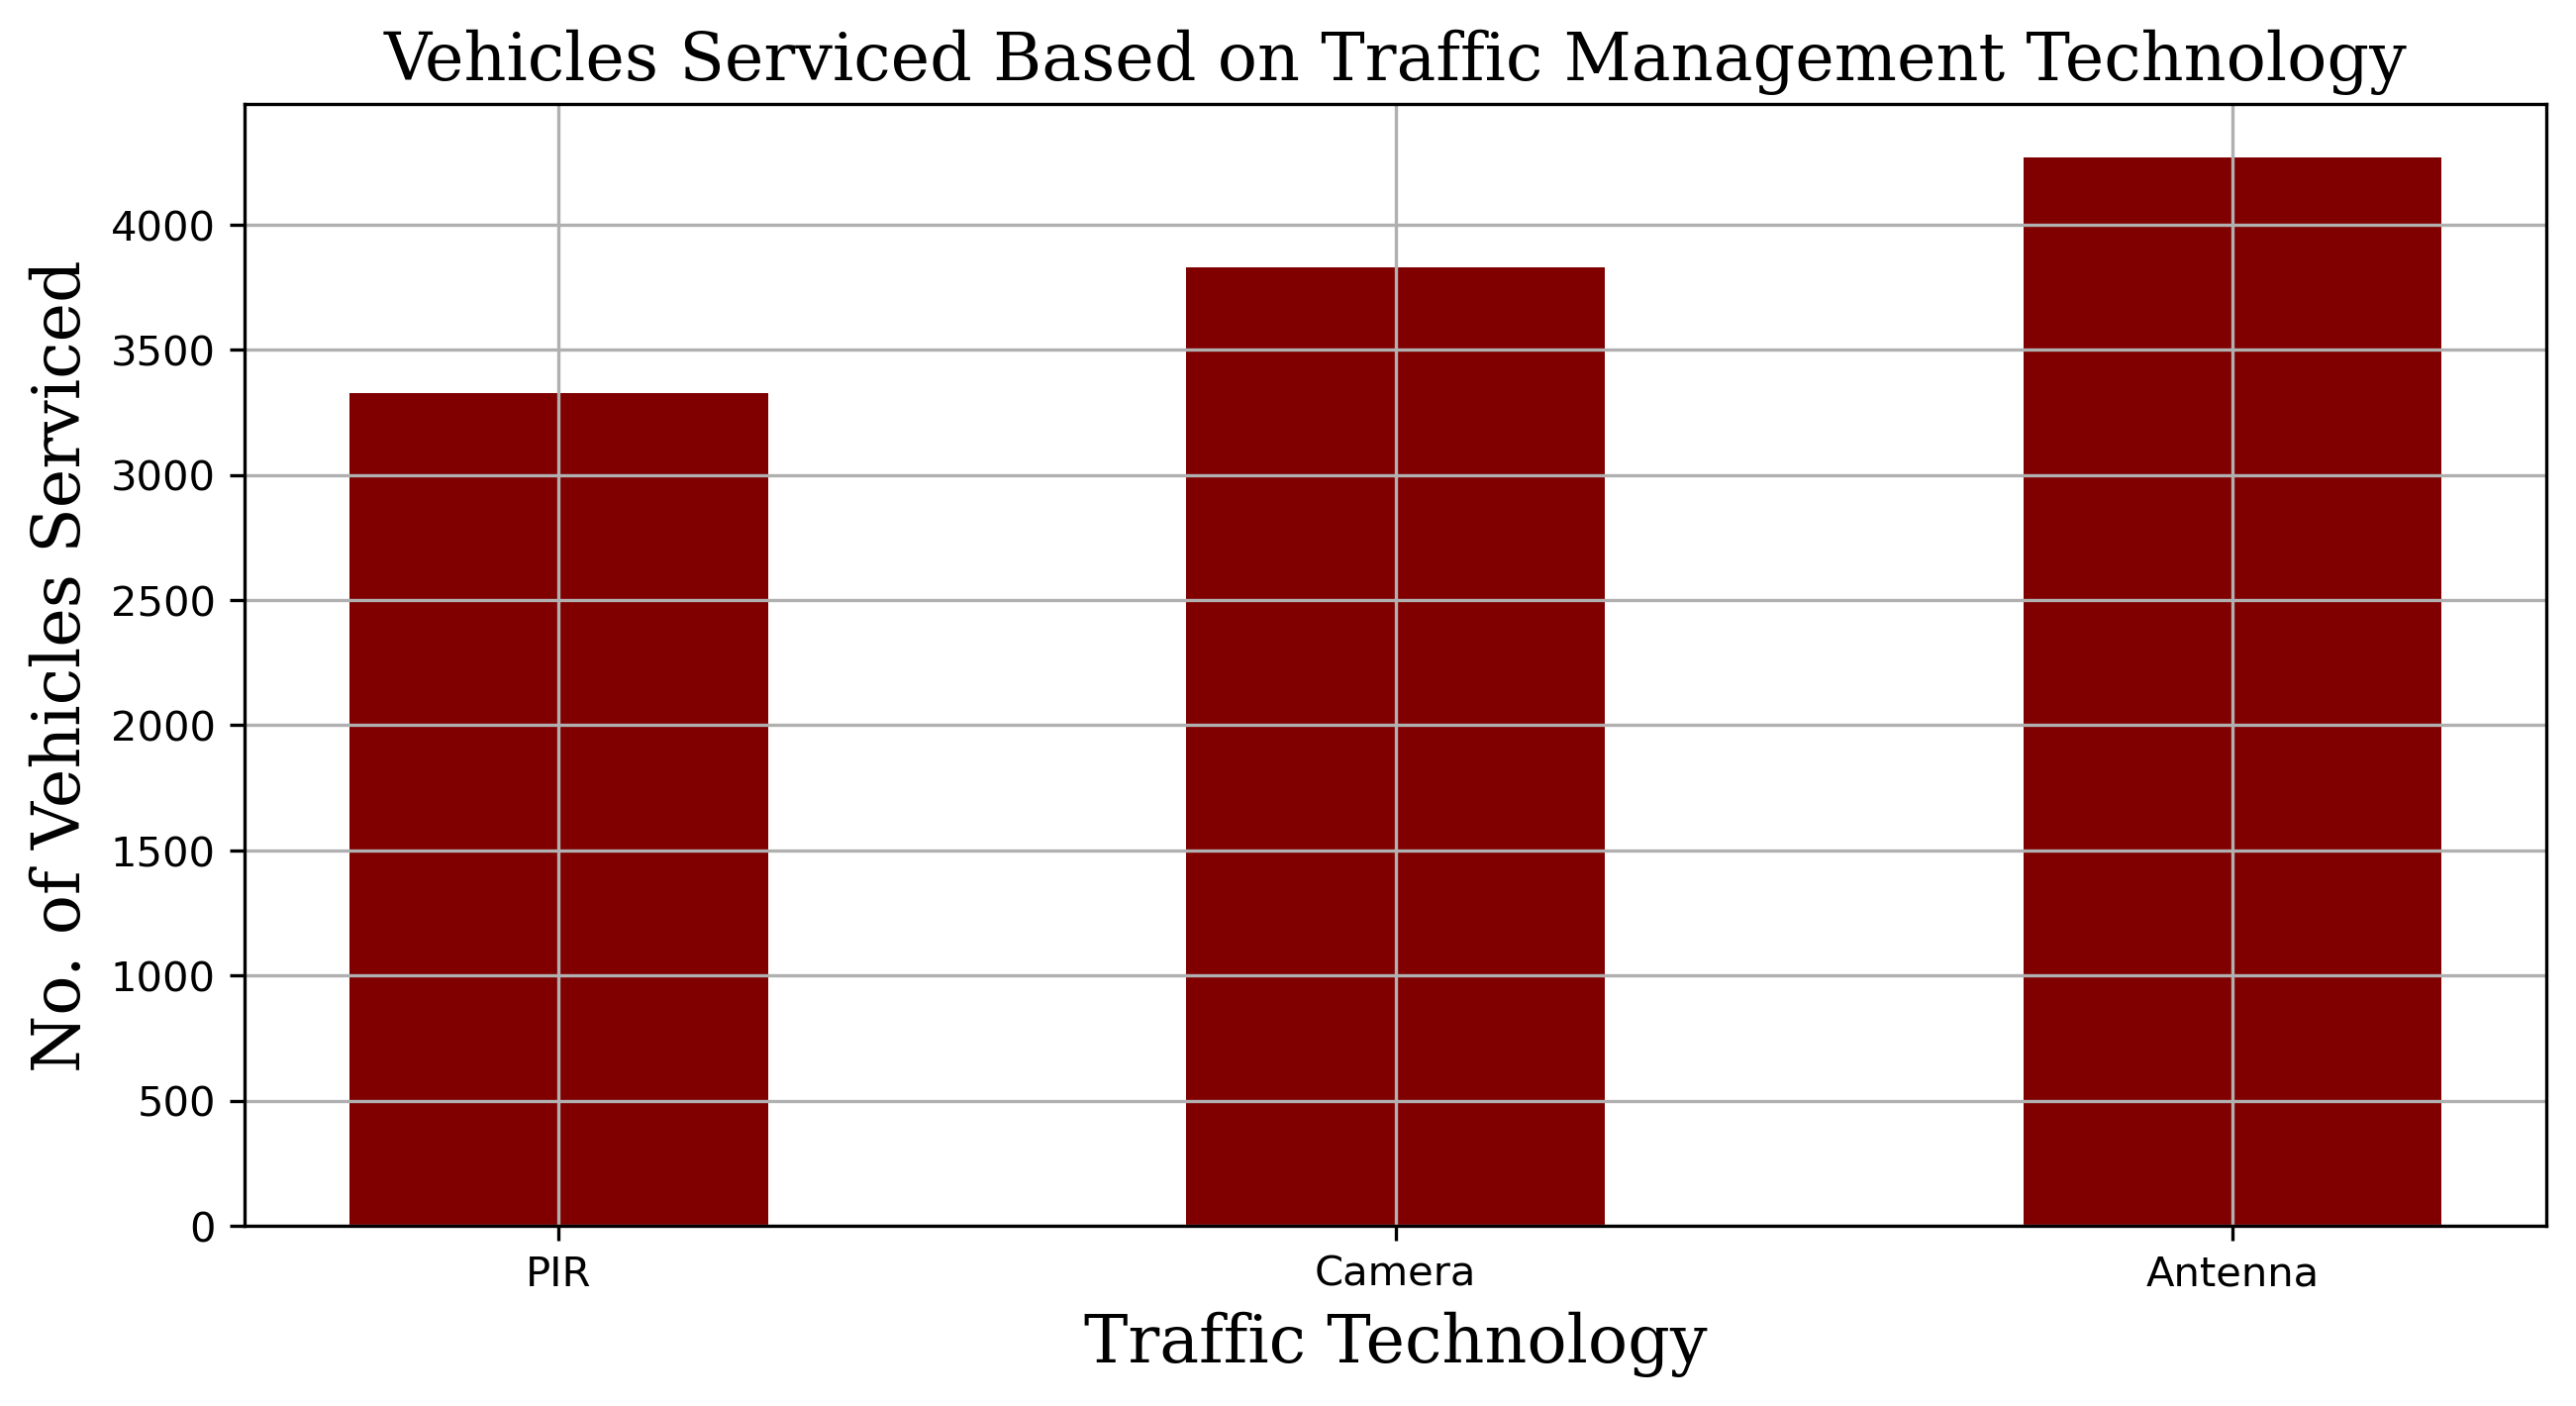
\includegraphics[width=\linewidth]{images/VehiclesServed_vs_Traffictechnology}
	\caption{Vehicles served based on traffic management technology.}
	\label{fig:vehiclesservedvstraffictechnology}
\end{figure}

Figure \ref{fig:vehiclesservedvstraffictechnology} shows the total number of cars served at the intersection during 1 hour of runtime, and organizes this information by traffic management technology. As shown above, the PIR sensor served 3,328 vehicles, the High Speed Camera served 3,828 vehicles, and the Smart Antenna served 4,267 vehicles.

\begin{figure}[H]
	\centering
	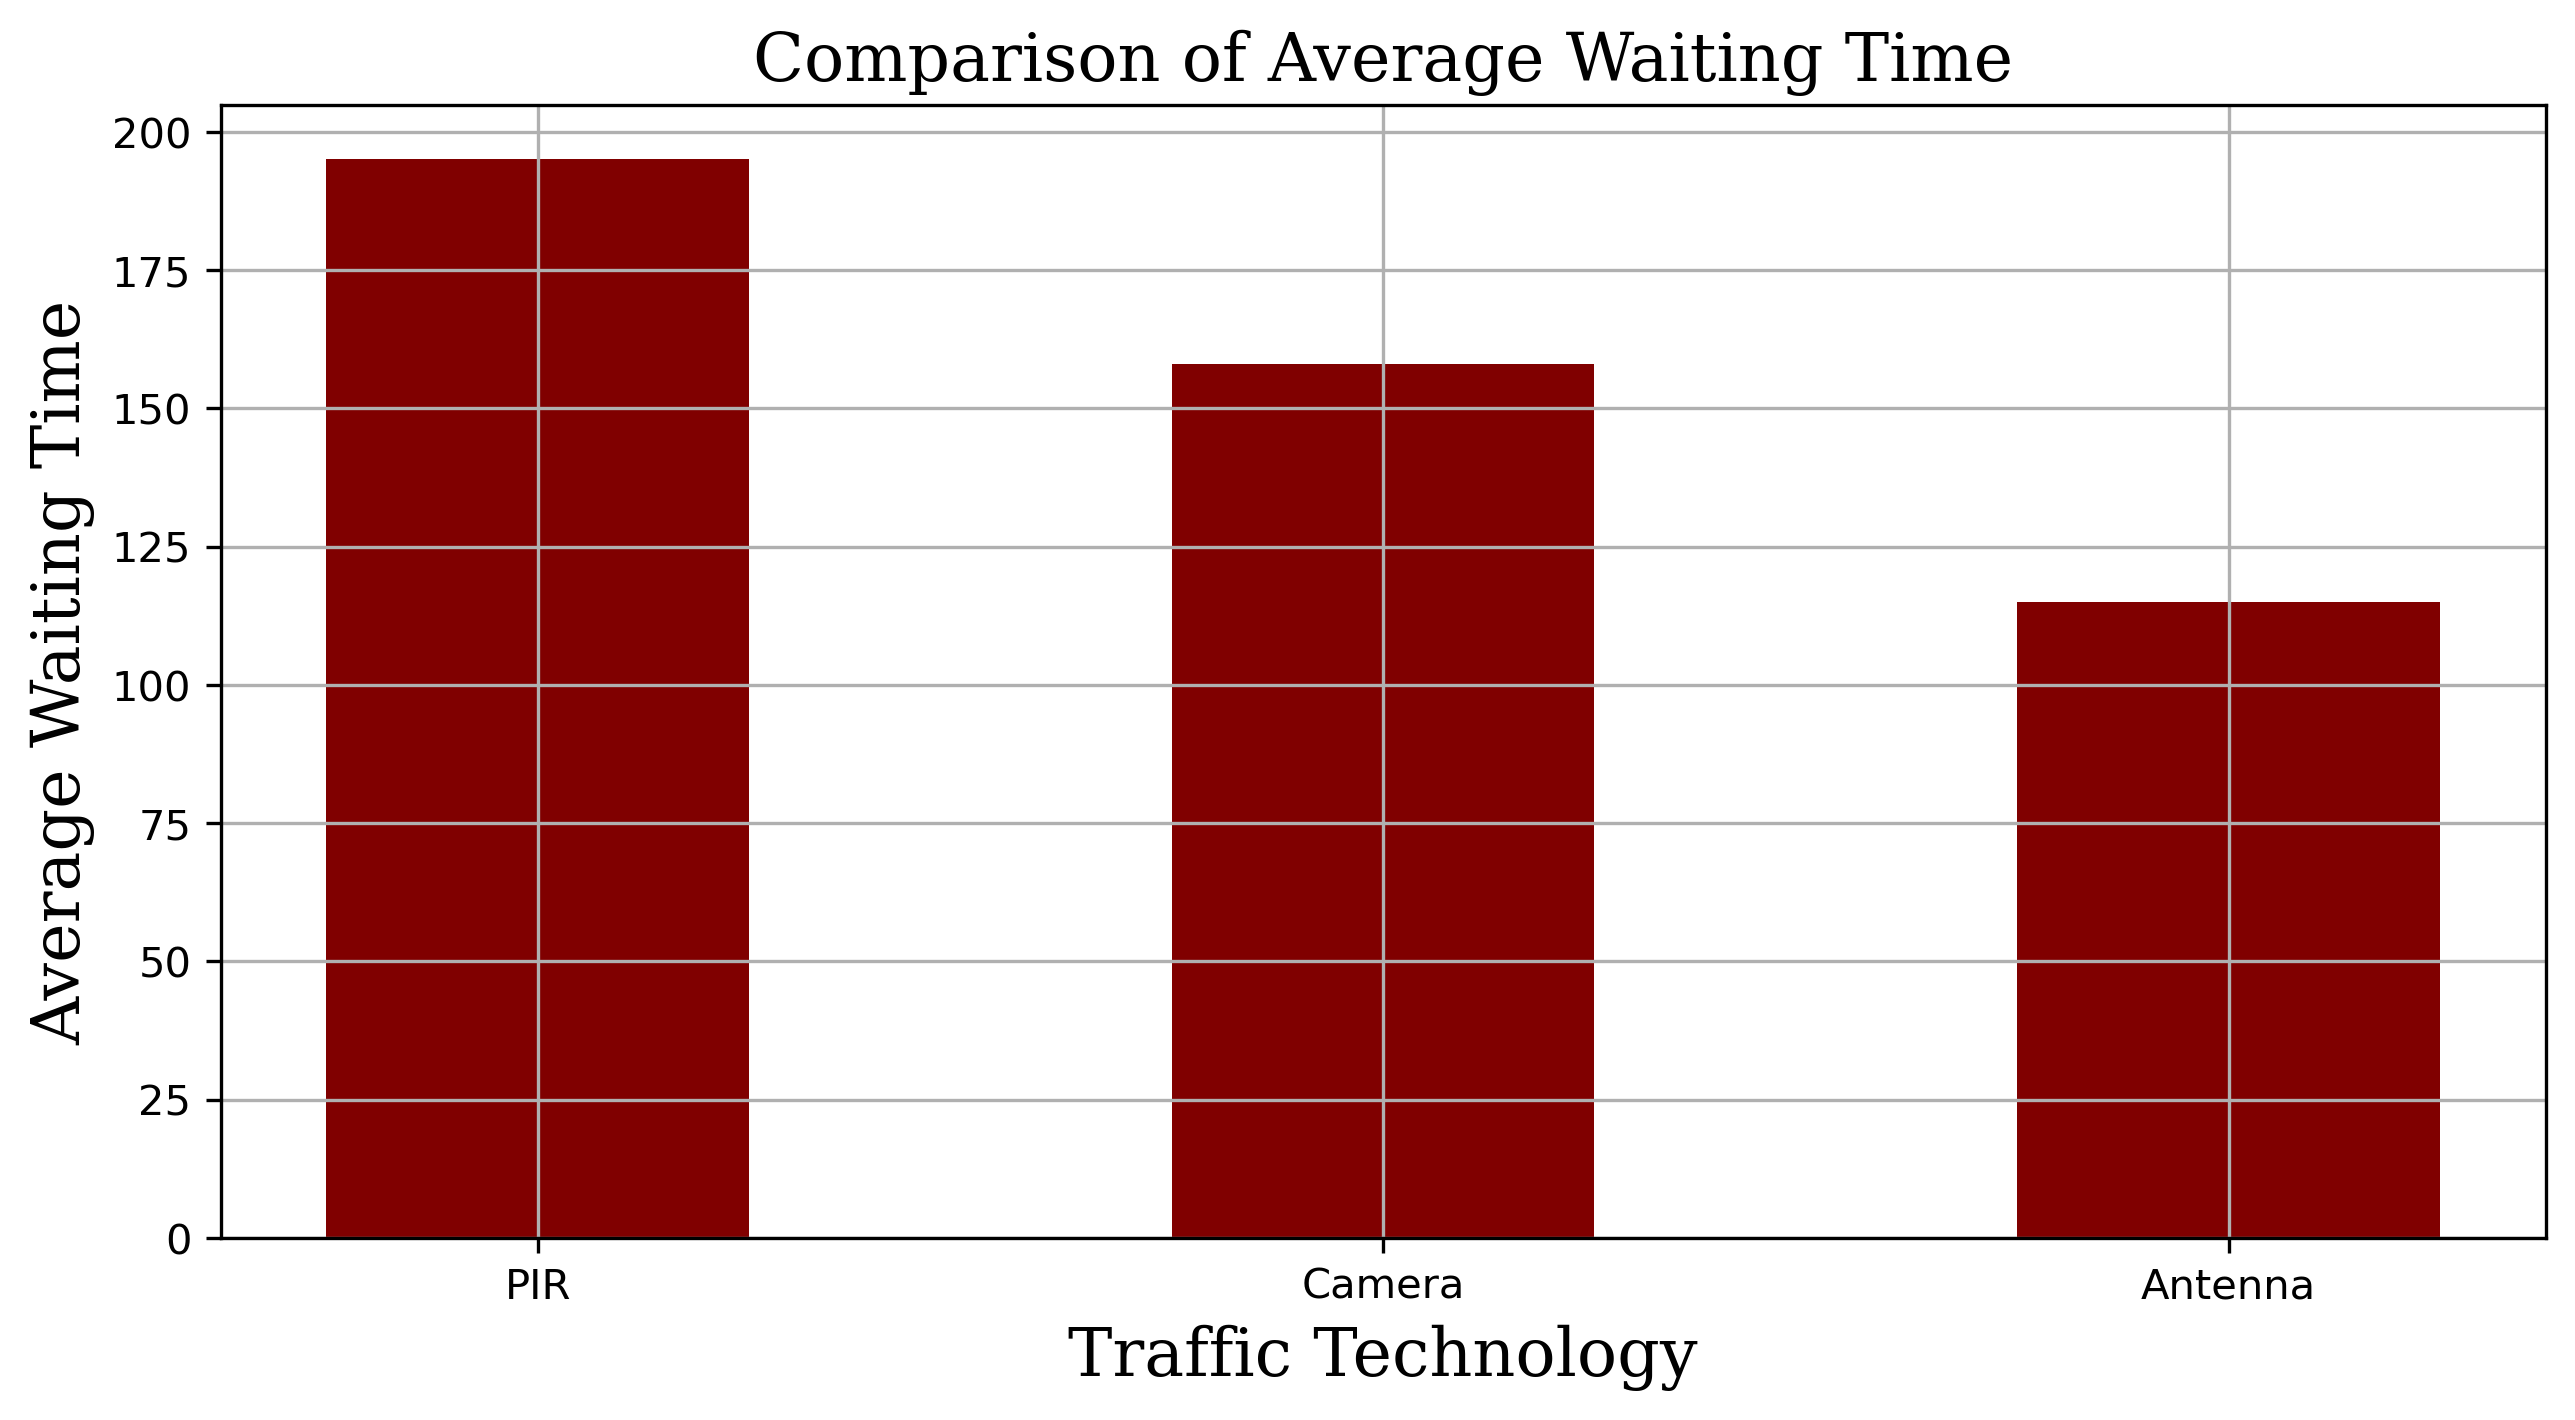
\includegraphics[width=\linewidth]{images/AWT_vs_TrafficTechnology}
	\caption{}
	\label{fig:awtvstraffictechnology}
\end{figure}

Figure \ref{fig:awtvstraffictechnology} compares the average waiting time at a red light experienced by the vehicles generated in the simulation environment. 

\begin{figure}[H]
	\centering
	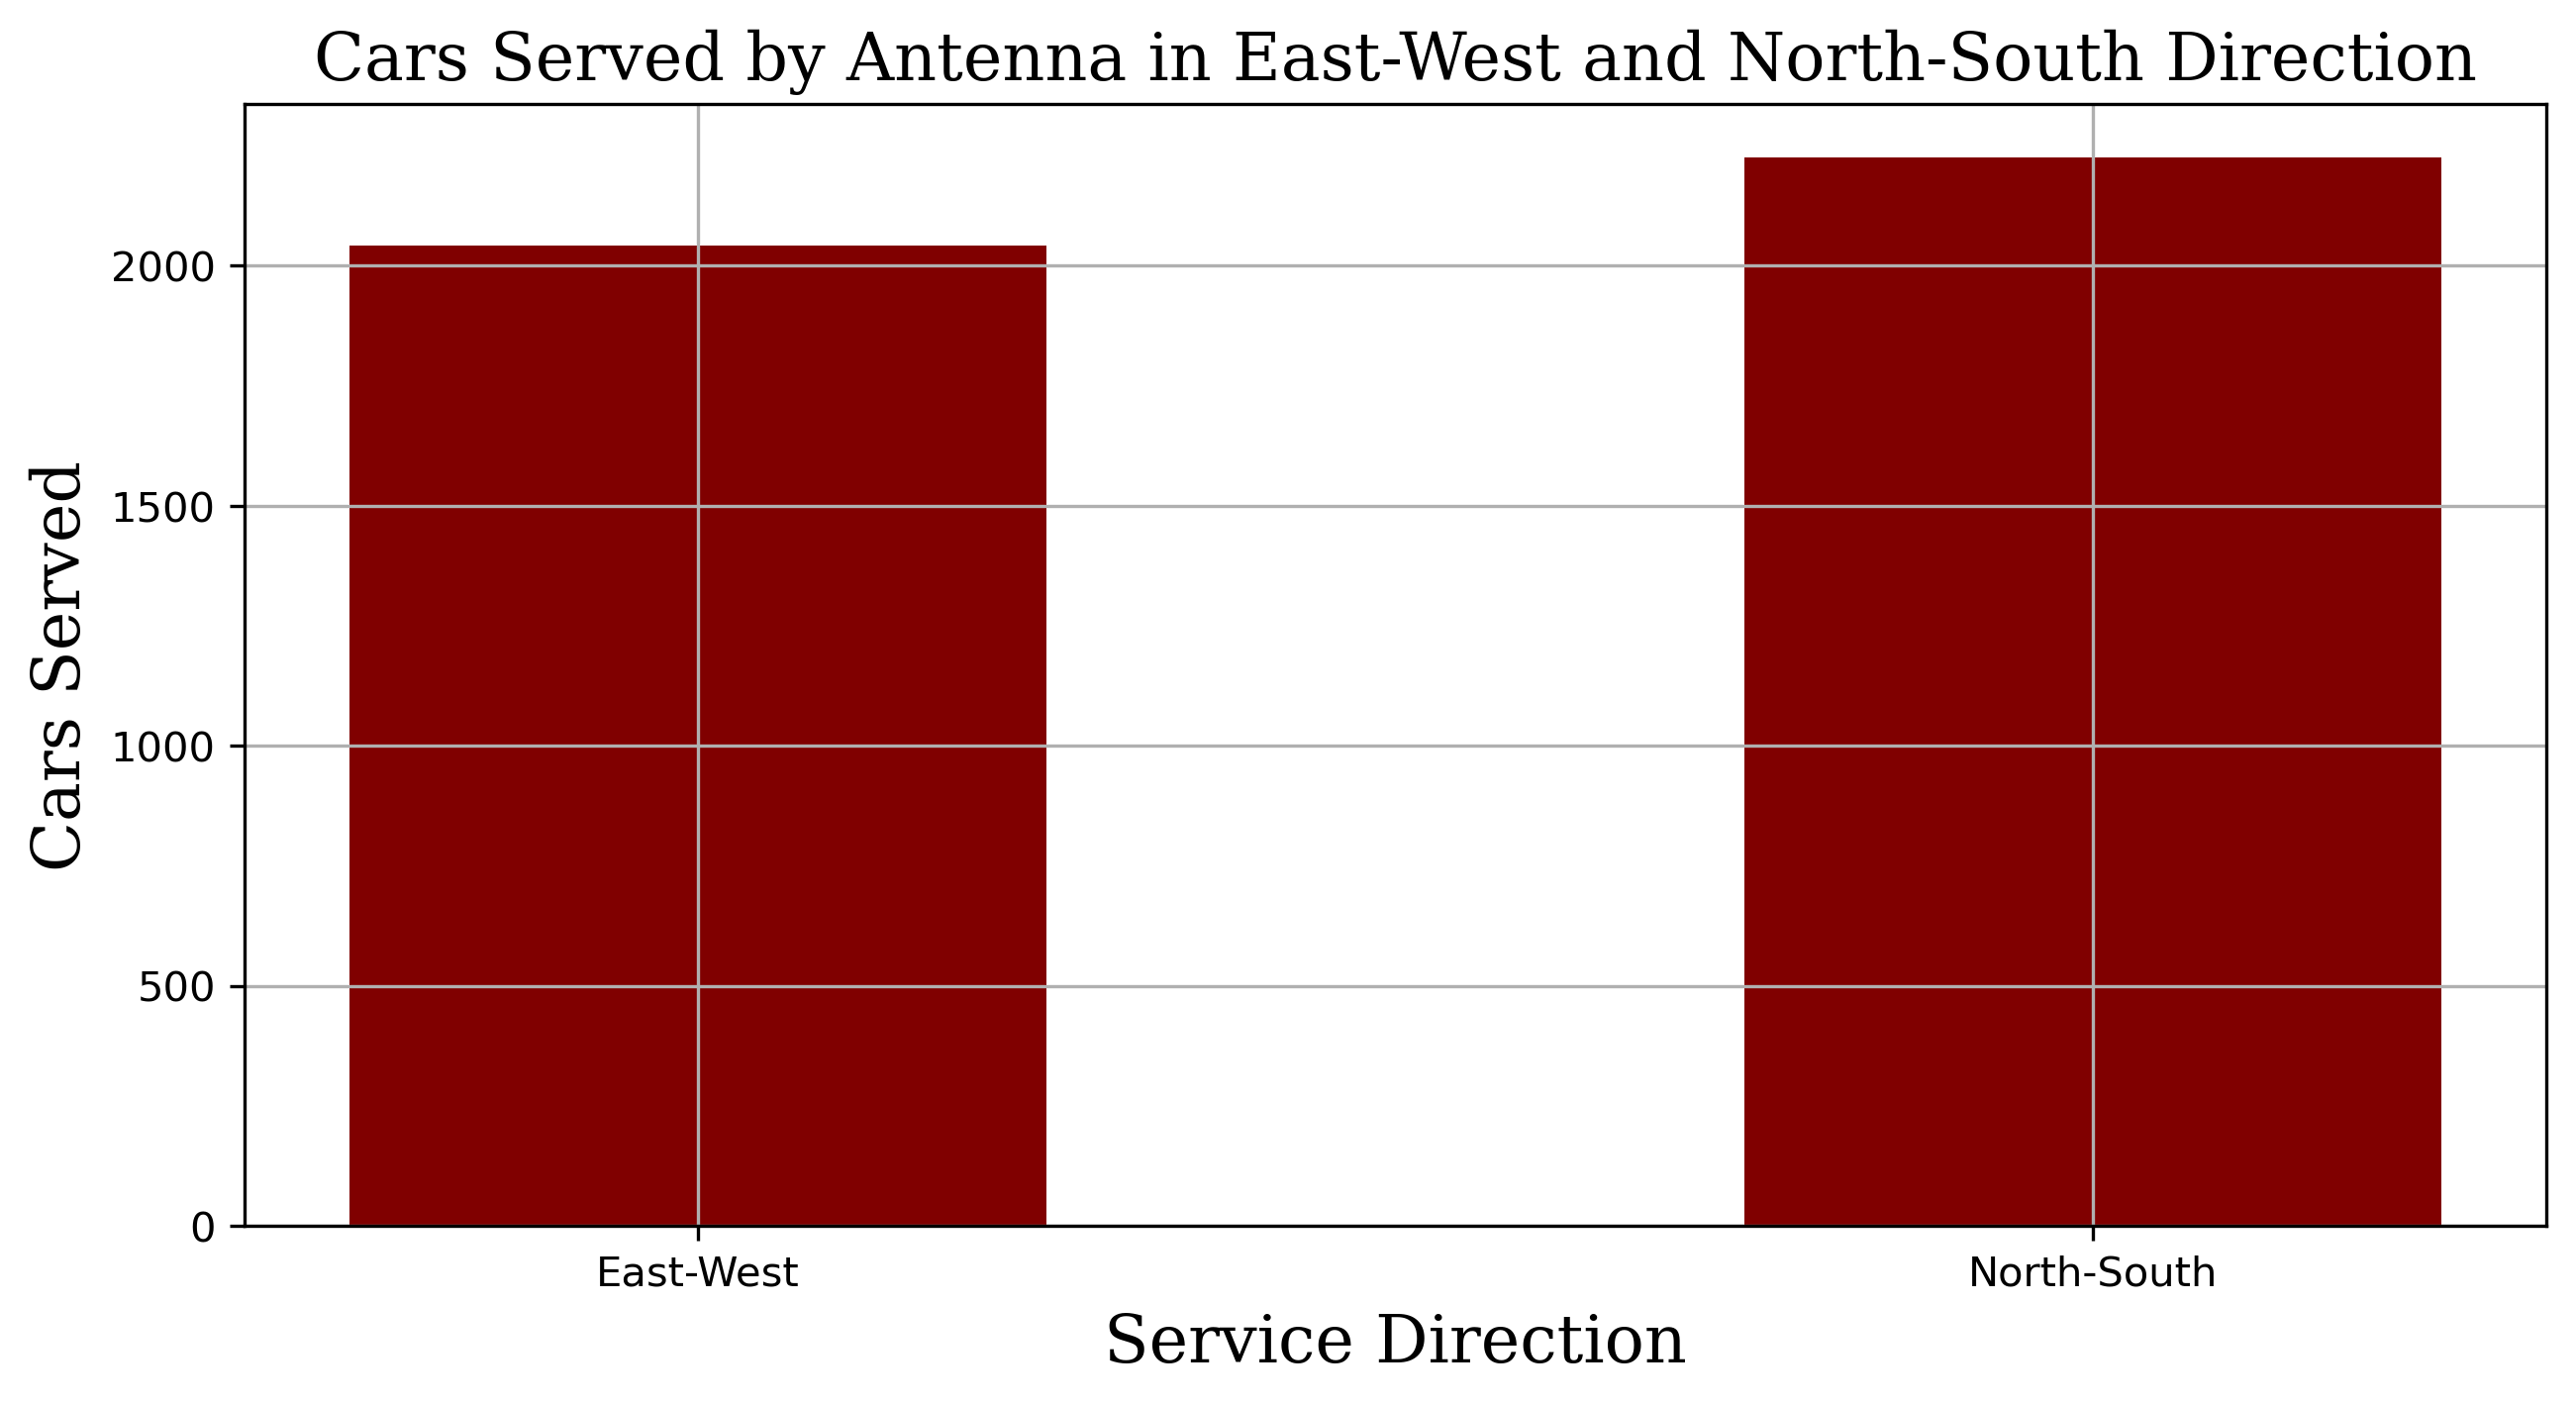
\includegraphics[width=\linewidth]{images/CarsServed_vs_Servicedirection}
	\caption{}
	\label{fig:carsservedvsservicedirection}
\end{figure}

Figure \ref{fig:carsservedvsservicedirection} shows the number of vehicles served by the Smart Antenna based on North to South and East to West directions.\\

\textbf{Data Analysis}

We ran the three simulations for 1 hour (3600 seconds) using the developed Python algorithms. In the simulations the traffic lights change dynamically depending on the number of cars present at the intersection using the logic explained in section \ref{sec_Methodology} for each technology.

\begin{figure}[H]
	\centering
	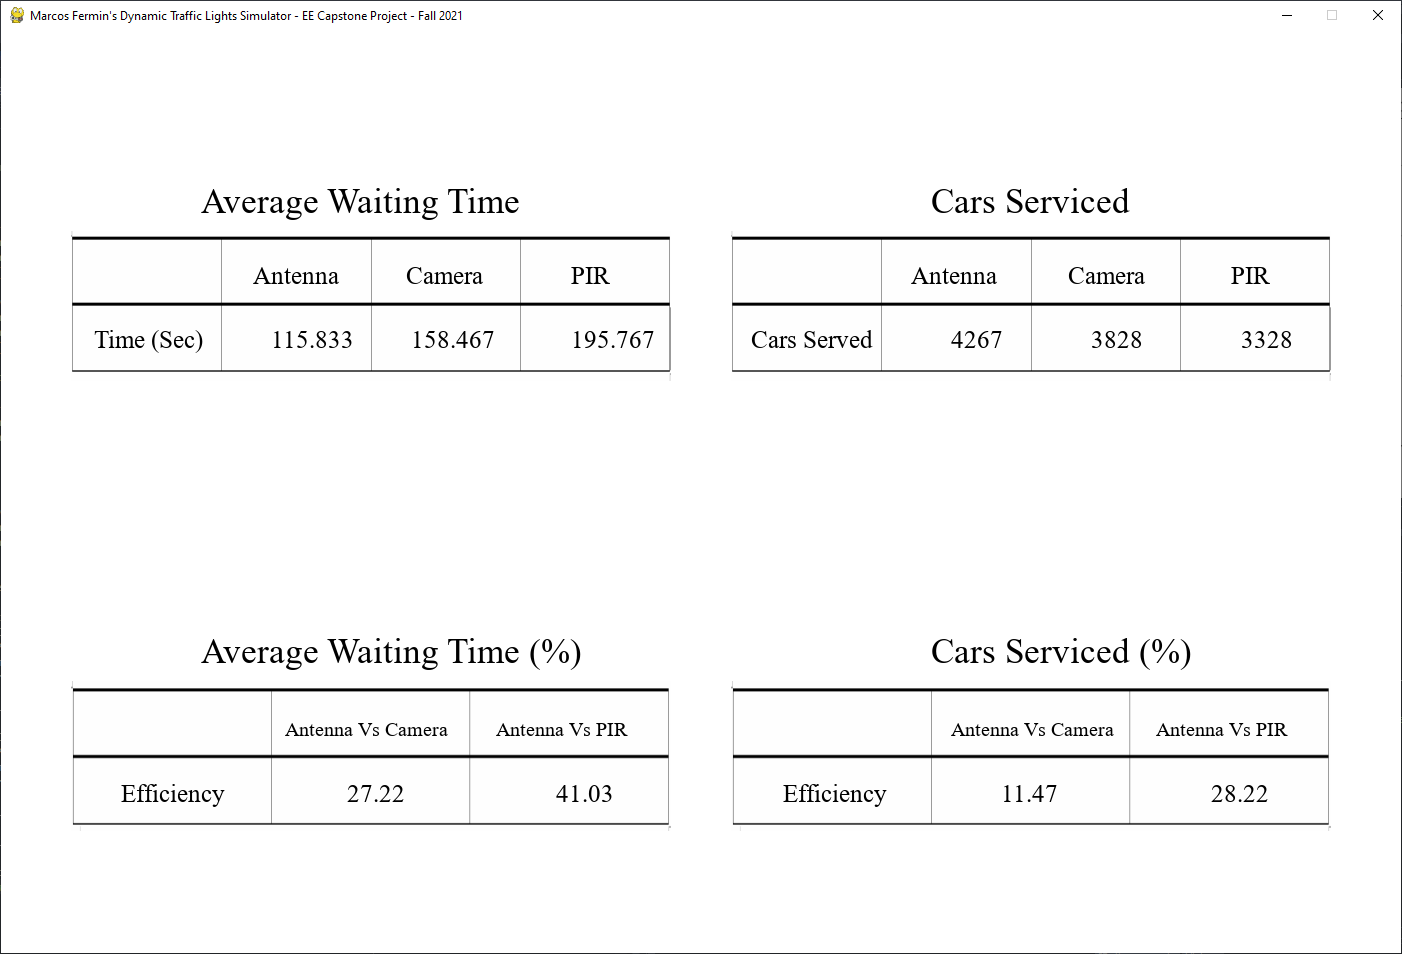
\includegraphics[width=\linewidth]{images/Tables}
	\caption{Tables comparing AWT, cars served and efficiency of each technology.}
	\label{fig:tables}
\end{figure}

In the simulation results shown in figure \ref{fig:tables} above, we can observe that during the Smart Antenna simulation the vehicles experienced an average waiting time of 115.833 seconds and 4,267 vehicles were served, in the High Speed Camera simulation vehicles experienced an average waiting time of 158.467 seconds and 3,828 vehicles were served, and that in the PIR sensor simulation vehicles experienced an average waiting time of 195.767 seconds and 3,828 vehicles were served.

From the obtained data we can determine the following:

\begin{itemize}
	\item The \textbf{Smart Antenna is more efficient at reducing congestion at the intersection} than the High Speed Camera and the PIR Sensor.
	\item The \textbf{Smart Antenna is 27.22\%} more efficient at reducing average waiting time than the High Speed camera, and \textbf{41.03\%} more efficient than the PIR Sensor. 
	\item The \textbf{Smart Antenna served 11.47\% more vehicles than the High Speed Camera}, and \textbf{28.22\% more vehicles than the PIR sensor}.
\end{itemize}


\newpage
%%%%%%%%%%%%%%%%%%%%%%%%%%%%%%%%%%%%%%%%%%%%%%%%%%%%%%%%%%%%%%%%%%%%%%%%%%%%%%%
\section{Conclusion}
\label{sec_Conclusion}

After completing this research project a microscopic simulation of a traffic flow model with Dynamic Traffic Lights using Pygame was developed. In this simulated environment the traffic lights timing self-adapts based on the traffic density at an arbitrary intersection. The performance of a smart antenna, high-speed cameras, and PIR sensors as distinct traffic management technologies in the simulated environment was compared, to determine which technology is more efficient at reducing congestion. Although real world traffic scenarios exhibit a high level of complexity, our simulations prove to be a reliable method of basic traffic flow modeling. After running the three simulations for 1 hour, we observed that the Smart Antenna is more efficient at reducing congestion at the intersection than the High Speed Camera and the PIR Sensor. We also observed that the Smart Antenna is 27.22\% more efficient at reducing average waiting time than the High Speed camera, and 41.03\% more efficient than the PIR Sensor. And that also the Smart Antenna served 11.47\% more vehicles than the High Speed Camera, and 28.22\% more vehicles than the PIR sensor. As demonstrated by the obtained results, the Smart Antenna is the superior traffic management technology.

\newpage
%%%%%%%%%%%%%%%%%%%%%%%%%%%%%%%%%%%%%%%%%%%%%%%%%%%%%%%%%%%%%%%%%%%%%%%%%%%%%%%

\section{Future Work}
\label{sec_future}

\begin{itemize}
	\item {\large Implement the Traffic Lights Controller in Real-Time using Computer Vision}
	\begin{itemize}
		\item Use Computer Vision algorithms to process the video image of the High Speed Camera and determine the real-time presence of vehicles and pedestrians at the intersections \cite{Rachmadi11}.
		\item Use NVIDIA Jetson Nano or Jetson AGX Xavier developer kits as the Computer Vision processing unit.
		\item Build a functional traffic light for real-time testing.
	\end{itemize}
\end{itemize}

\begin{itemize}
	\item {\large Create a Physical Traffic Lights Controller with PIR Sensor using IoT Embedded Board}
	\begin{itemize}
		\item Create a physical Traffic Lights Controller by programming an open-source dedicated IoT Embedded Board (FPGA, Arduino, Raspberry Pi, etc).
		\item Create a model of an intersection and place a PIR sensor at the corners to sense vehicles' motion. 
		\item Optimize Traffic Lights Timing based on PIR sensor readings \cite{Zachariah17}. 
	\end{itemize}
\end{itemize}

\newpage
%%%%%%%%%%%%%%%%%%%%%%%%%%%%%%%%%%%%%%%%%%%%%%%%%%%%%%%%%%%%%%%%%%%%%%%%%%%%%%%
%%%%%%%%%%%%%%%%%%%%%%%%%%%%%%%%%%%%%%%%%%%%%%%%%%%%%%%%%%%%%%%%%%%%%%%%%%%%%%%
%%%%%%%%%%%%%%%%%%%%%%%%%%%%%%%%%%%%%%%%%%%%%%%%%%%%%%%%%%%%%%%%%%%%%%%%%%%%%%%
\section{References}
\label{sec_references}

\begin{singlespace}  % use single-line spacing for multi-line text within a single reference
	\setlength\bibitemsep{\baselineskip}  %manually set separation between items in bibliography to double space
	\printbibliography[heading=none]
\end{singlespace}

\newpage
%%%%%%%%%%%%%%%%%%%%%%%%%%%%%%%%%%%%%%%%%%%%%%%%%%%%%%%%%%%%%%%%%%%%%%%%%%%%%%%

\section{Appendix: Python Codes}
\label{sec_codes}

\subsection{Github}

To access this project on Github scan the QR Code below:

\begin{figure}[H]
	\centering
	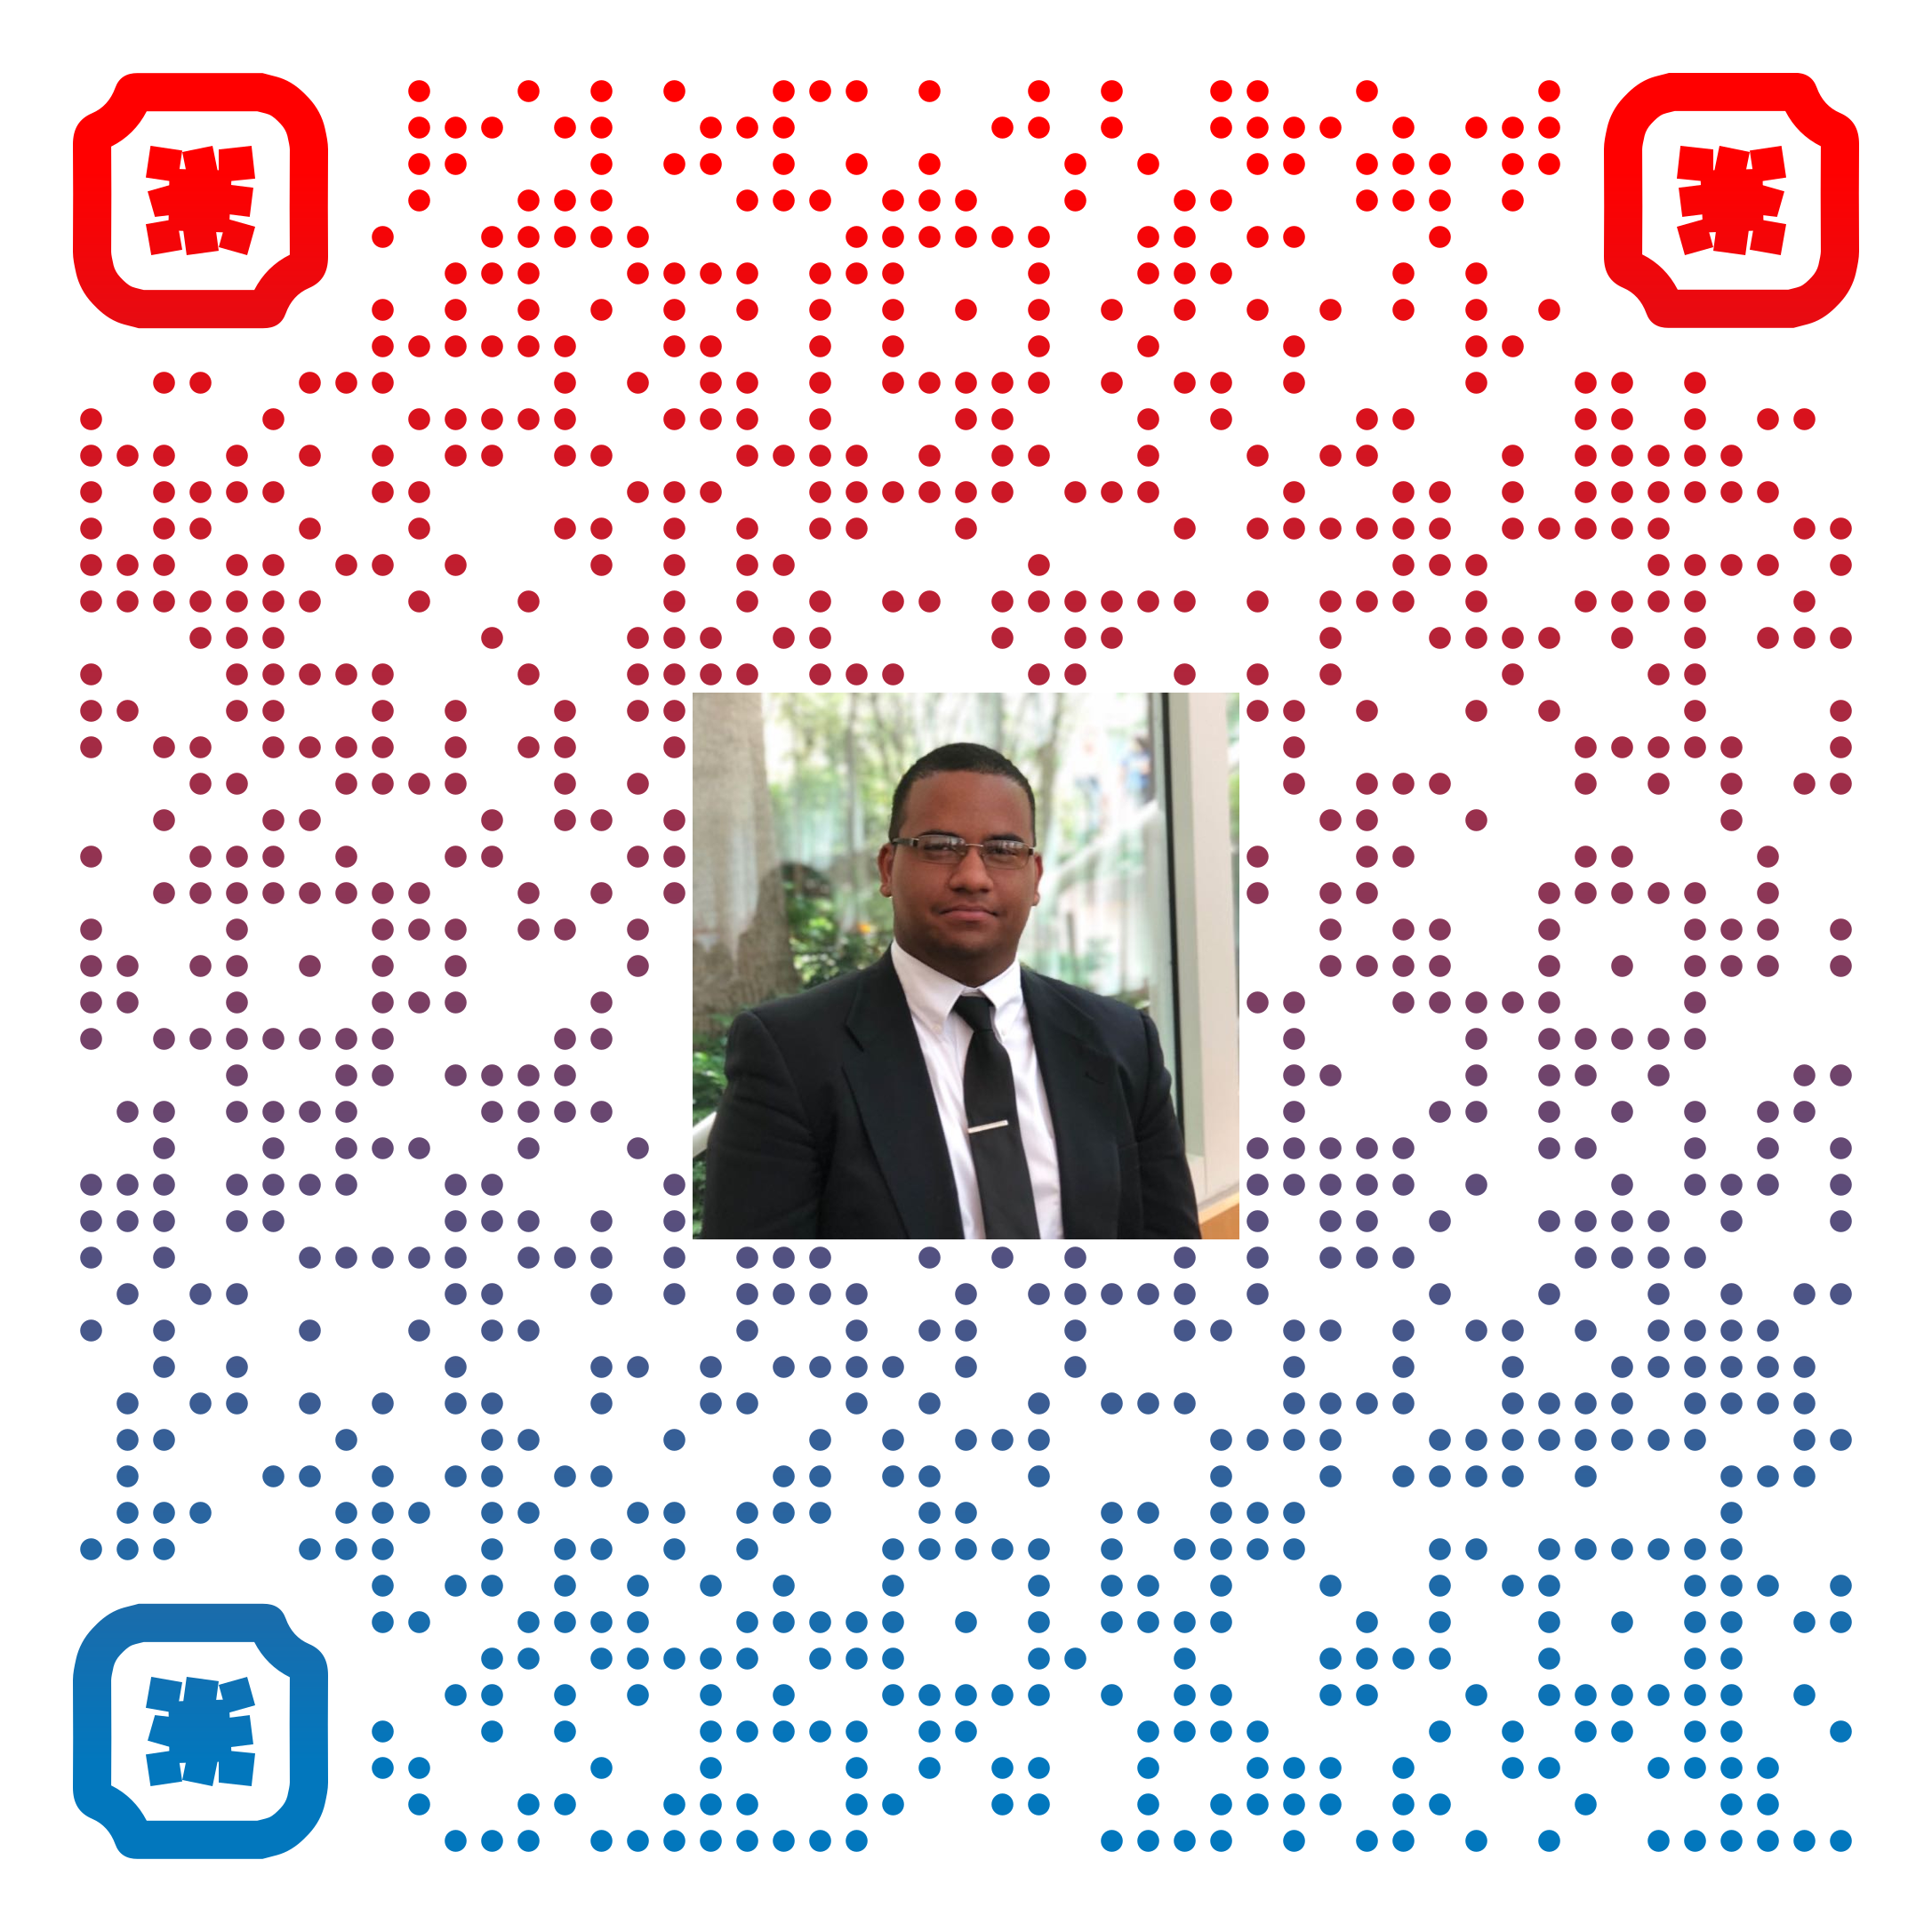
\includegraphics[width=.9\linewidth]{images/qr-code}
	https://github.com/marcostfermin/Dynamic-Traffic-Lights-Simulation
	\label{fig:qr-code}
\end{figure}

%%%%%%%%%%%%%%%%%%%%%%%%%%%%%%%%%%%%%%%%%%%%%%%%%%%%%%%%%%%%%%%%%%%%%%%%%%%%%%%

\clearpage
\end{document}

